\documentclass[]{final_report}
\usepackage{graphicx}
\usepackage{hyperref}
\usepackage{titlesec}
\usepackage[utf8]{inputenc}
\usepackage[backend=biber, style=ieee]{biblatex}
\usepackage{amsmath}
\usepackage{amssymb}
\usepackage{float}
\usepackage{tabularx} % Needed for the X column type
\usepackage{booktabs} % For prettier tables
\usepackage{lipsum}   % For dummy text
\usepackage{mathtools}
\usepackage{stmaryrd}
\usepackage{mdframed}
\usepackage{caption}
\usepackage{array}
\usepackage{listings}
\usepackage[dvipsnames]{xcolor}
\usepackage{adjustbox}
\usepackage{tikz}
\usepackage{rotating}
\usepackage{pdflscape}
\usepackage{fancyhdr}
\usepackage{comment}
\usepackage{array}
\usepackage{multirow}
\usepackage{tcolorbox} 
\fancypagestyle{lscape}{%
  \fancyhf{} % clear all header and footer fields
  \fancyfoot[LE,RO]{\makebox[0pt][l]{\rotatebox[origin=c]{90}{\thepage}}} % Left Even, Right Odd
  \renewcommand{\headrulewidth}{0pt}
  \renewcommand{\footrulewidth}{0pt}
}


\addbibresource{fyp.bib}
\usepackage{amsthm}
\theoremstyle{definition}
\newtheorem{definition}{Definition}[chapter]
\newtheorem{basic}{Basic Definition}
\newtheorem{theorem}{Theorem}
\newtheorem{implication}{Implication}

% Define the Java code style
\lstdefinestyle{mystyle}{
    language=Java,
    commentstyle=\color{OliveGreen},
    keywordstyle=\color{blue},
    numberstyle=\tiny\color{gray},
    stringstyle=\color{red},
    basicstyle=\ttfamily\footnotesize,
    breakatwhitespace=false,         
    breaklines=true,                 
    captionpos=b,                    
    keepspaces=true,                 
    numbers=left,                    
    numbersep=5pt,                  
    showspaces=false,                
    showstringspaces=false,
    showtabs=false,                  
    tabsize=2
}
\lstset{style=mystyle}

\newcommand{\mycomment}[1]{}
%%%%%%%%%%%%%%%%%%%%%%
%%% Input project details
\def\studentname{Jude Asare}
\def\reportyear{2023/2024}
\def\projecttitle{Implementing the PKCS\#1 v1.5 Signature Scheme with provably secure parameters}
\def\supervisorname{Saqib Kakvi}
\def\degree{MSci (Hons) in Computer Science (Information Security)}
\def\fullOrHalfUnit{MSci} 
\def\finalOrInterim{Interim Report} 
\begin{document}

\maketitle





%%%%%%%%%%%%%%%%%%%%%%
%%% Table of Contents
\tableofcontents\pdfbookmark[0]{Table of Contents}{toc}\newpage



%%%%%%%%%%%%%%%%%%%%%%
%%% Your Abstract here
\begin{comment}
\mycomment{

\begin{abstract}



The PKCS\#1 v1.5 digital signature scheme has been widely utilised in protocols such as SSH, DNSSEC, IKE, and most prominently, in TLS up to version 1.2. Since its inception in 1998 \cite{rfc2313} it has played a pivotal role in the landscape of digital security comprising the most widely used digital signature scheme in practice. The scheme, renowned for its straightforwardness and expedited verification capabilities, has seen persistent integration across diverse cryptographic systems. 

Nevertheless, amidst its widespread acceptance, it's been marred by several challenges. Among these are the targeting of a latent vulnerability with incorrectly implemented signature verification implementations \cite{finney2006bleichenbacher, kuhn2008variants, bock2018return} stemming from attacks \cite{bleichenbacher1998chosen} exploiting its provably insecure associated encryption paradigm \cite{rfc2313} and a glaring absence of a rigorous security proof that validates its robustness.

Even though alternatives like RSA-PSS offer provable security (\cite{bellare1996exact}, \cite{jonsson2001security}), they come with inherent problem, such as the introduction of randomness and a hike in computational complexity. These issues have created reservations for its wholesale adoption in place of PKCS\#1 v1.5 e.g., RSA-PSS and was only upgraded to a requirement for new applications in PKCS\#1 v2.2 \cite{rfc8017} long after initially being suggested as the replacement for PKCS\#1 v1.5 in PKCS\#1 v2.1 \cite{rfc3447}. Imperative requirements of backward compatibility and interoperability have been the main detractors of the aversion to replacing PKCS\#1 v1.5 and while RSA-PSS is now required in new applications, they entail retaining PKCS\#1 v1.5 in some form at the very least, as a preferable choice.
 
A significant breakthrough came in 2018 when Jager, Kakvi, and May \cite{jager2018security} provided a security proof for the PKCS\#1 v1.5 Signature scheme building on the work of Coron \cite{coron2002security}. Although still requiring the adoption of larger cryptographic parameters deviating slightly from standard use, their methods were flexible enough to show instantiations in practice such that the improved proofs apply. Benefits not limited to PKCS\#1 v1.5, their work also offered insights enabling the proof to apply to other deterministic RSA signature schemes, with similar construction patterns including ISO/IEC 9796-2 and ANSI X9.31 schemes.

Guided by this revelation, this project seeks to concretely implement these signature schemes, with a primary emphasis on the PKCS\#1 v1.5 signature scheme, using the aforementioned provably secure parameters. This project primarily aims to dissect the computational burdens these parameters introduce into deterministic RSA schemes. This aim is supplemented by supporting objectives to produce algorithms that facilitate its implementation with provably secure parameters and standard parameters. From there the main objective is to produce a user-interfaced benchmarking program to explore aforementioned overhead across standards. 
\newpage
\end{abstract}
}
\end{comment}
\newpage


%%%%%%%%%%%%%%%%%%%%%%
%%% Introduction
\chapter{Introduction}


\section{Aims}

\subsection{Why: The Context and Rationale}
The PKCS\#1 v1.5 digital signature scheme, rooted in RSA's hash-and-sign framework, has emerged as the de facto standard for digital signatures since its 1998 introduction \cite{rfc2313}. Essential in security-focused network protocols like SSH, DNSSEC, IKE, and pre-TLS 1.3 X.509 certificates \cite{schaad2005additional}, its simplicity fostered broad adoption from its outset with a straightforward implementation across programming languages, and speedy verifications relative to alternatives like DSA or ECDS  \cite{jager2018security}. 
Despite its widespread adoption the scheme lacks formal security proofs, raising concerns about its long-term reliability.
Given its deep integration in various applications, even at the hardware level, transitioning to provably secure \cite{bellare1996exact, jonsson2001security} alternatives like RSA-PSS has been slow (RSA-PSS was only upgraded to a requirement for new applications in PKCS\#1 v2.2 \cite{rfc8017} long after initially being suggested as the replacement for PKCS\#1 v1.5 in PKCS\#1 v2.1 \cite{rfc3447}) with imperative requirements of backward compatibility and interoperability acting as significant barriers to full adoption.

Additionally considered in a broader sense, for a cryptographic scheme i.e., RSA-PSS to gain traction it must first be developed and then subjected to rigorous scrutiny by the cryptographic community. Following this, its algorithmic primitives need to be standardised, which then facilitates the creation and standardisation of high-level protocols incorporating these components. Subsequent software implementations must align with these standards before the scheme can be set as the default in various applications. RSA-PSS, while superior to the older PKCS\#1 v1.5 lingers in the early stages of this transition mainly between standardisation of its algorithm primitives and the standardisation of protocols that incorporate its primitives. The current landscape is one of fragmentation where RSA-PSS and PKCS\#1-v1.5 often coexist within the same infrastructure, such as TLS implementations and RSA certificates. This state of the art considered, retaining PKCS\#1 v1.5 scheme remains a preferable choice. Going even further, finding an applicable security proof to bridge its security to the level of its widespread adoption would be the ideal scenario.

In this direction a landmark development came in 2018 when Jager, Kakvi, and May \cite{jager2018security} provided a security proof (an improvement on Coron proof that was limited to the Rabin-Williams variant with e=2 \cite{coron2002security}) for the PKCS\#1 v1.5 signature scheme, with a caveat: usage of larger parameters are required. Their work offered insights that also apply to other deterministic RSA signature schemes, including ISO/IEC 9796-2 Scheme and ANSI X9.31.

\subsection{What: The Primary Goal}
The aim of this project was to connect the theoretical concepts introduced by Jager et al. \cite{jager2018security} with practical application. This involved implementing and then assessing the computational burden that arises when using provably secure parameters in deterministic RSA signature schemes, particularly within the context of the PKCS standard.

\subsection{How: Overview of Objectives}
The influence of the application of provably secure parameters to each of the mentioned deterministic schemes in terms of computational cost was investigated. This was done through the production of algorithms respective to both cases (standard and provably secure parameters) allowing for comparison. Performing the investigation across standards was means of ascertaining a more reliable and accurate assessment by enabling further comparison of introduced overhead across different schemes. The final deliverable constituted an all-incorporative user-interfaced benchmarking program for which results from automation of signature processes applied to data were generated for appropriate evaluations and conclusions to be drawn.


\section{Objectives}
To achieve the aim, the project will involve:
\begin{itemize}
    \item Exploring the security proof relevant to the PKCS\#1 v1.5 signature scheme .
    \item Determining the practical implications arising from the security proof on instantiations of the full suite of deterministic signature schemes (PKCS\#1-v1.5, ISO/IEC-9796-2, and ANSI-X9.31 signature schemes).
    \item Developing concrete implementations of the considered deterministic signature schemes using standard and provable parameters.
    \item Demonstrating in practice, with larger parameters, how deterministic schemes can achieve a security level on par with less-practical, signature schemes, such as RSA-PSS.
      \item Evaluating and comparing computational performance of instantiating the considered signature schemes with standard vs. provable parameters. 
     \item Creating a user-interfaced benchmarking program that incorporates all objectives of the project to assess this overhead in various scenarios across and within standards.

\end{itemize}



 
\chapter{Literature Review/Related Work}
RSASSA-PKCS1-v1.5 remains unbroken. There are no real attacks able to successfully exploit the scheme free of implementation errors. This distinction of being free of implementation errors is crucial. Potential proofs consider only forgeries that are accepted by a correct verification algorithm. It is now well established from a variety of follow up studies all originating from \cite{bleichenbacher1998chosen} that vulnerable implementations of a flawed signature verification algorithm for RSASSA-PKCS1-v1.5 can be exploited. Bleichenbacher presented a low-exponent attack on RSA-PKCS\#1 v1.5 signatures at the CRYPTO 2006 rump session. This attack was later described by Finney \cite{finney2006bleichenbacher} in a posting to the OpenPGP mailing list. 

It was not until the efforts of Coron in 2002 (\cite{coron2002security}) that a security proof applicable to RSASSA-PKCS1-v1.5 arrived. This was due to the issue of deterministic padding scheme that RSASSA-PKCS1-v1.5 uses rendering standard proof techniques void. Coron presented a security proof for RSASSA-PKCS1-v1.5 (and ISO/IEC 9796-2 signatures) albeit with a restriction that e = 2, i.e. the Rabin-Williams variant \cite{coron2002security} which is secure based on the factoring assumption. 
The proofs' exclusive and/or restrictive value of e aside, a further caveat was that the output size of the hash function needed to be 2/3 of the bit length of the modulus N. These restrictions diverge largely from the parameters used in the instantiation of RSA-PKCS\#1 v1.5 signatures in practice. 

Much later, Jager, Kakvi and May \cite{jager2018security} showed an improved security proof for RSASSA-PKCS1-v1 5 with less restrictive conditions.
It sufficed that e more generally be a small prime (Kakvi and Kiltz \cite{kakvi2018optimal}). Still requiring a large hash function output, Jager, Kakvi and May achieved an improvement in hash function output requiring only 1/2 of the modulus size. The modulus effectively doubles in bit length when compared to the norm with a newly introduced third prime factor necessitating the increase in bits.
Withstanding the improvement and as a consequence of the proofs being founded in the random oracle model, the larger cryptographic parameters still deviate slightly from the standard parameters used in practice. Nonetheless this was sufficient enough for the authors to demonstrate how RSA-PKCS\#1 v1.5 signatures can be instantiated in practice such that the improved proofs apply. 

To all intents and purposes, regardless of the proofs being presented primarily for RSASSA-PKCS1-v1.5, uniformity in construction philosophy means other signature standards of the same deterministic RSA type (ISO/IEC 9796-2 signatures and ANSI X9.31 rDSA) still match the setting required for proofs to be applicable to them. For example theorem statements used in construction of Corons' proof \cite{coron2002security} are general enough that corresponding proof theorems can also be presented for the remaining standards of deterministic signatures. 

A full discussion of provable security extending to non-deterministic schemes lies beyond the scope of this project. Probabilistic padding poses an issue since generating sources of randomness, particularly on constrained devices is an ongoing challenge. Moreover RSA-PSS, the sole RSA-based randomised digital signature scheme uses two hash functions. This makes it difficult to compare with deterministic schemes that use only one. This project focused on standardised deterministic schemes which are directly comparable and subversion resistant \cite{ateniese2015subversion} by default of not having to generate randomness. This lends well to the issue of examining computational overhead from various perspectives of the different deterministic standards.



\chapter{Cryptographic Foundations}
\section{Notations}
The security parameter is denoted as \( \lambda \). 
This parameter determines a system's security level or key sizes. A larger value of $\lambda$ indicates stronger security, though it requires more computational effort. The concept of binary strings is frequently referred to. Specifically for all \( n \in \mathbb{N} \), the symbol \( 1^n \) represents the n-bit string of consecutive ones. 

In cryptographic operations, sampling often involves randomness. Given any set \( S \), the notation \( x \in_{R} S \) signifies that \( x \) is chosen uniformly at random from \( S \).  
The set of prime numbers is represented as \( \mathbb{P} \) and the set of \( k \)-bit primes is denoted as \( \mathbb{P}[k] \). Similarly, the set of integers is represented by \( \mathbb{Z} \) and \( \mathbb{Z}[k] \) respectively. 

The notation \( \mathbb{Z}_N^* \) represents the multiplicative group modulo \( N \) where \( N \in \mathbb{N} \). 

Finally, game-based proofs are employed, and the notation \( G^A \Rightarrow 1 \) indicates an event where the adversary \( A \) succeeds in game \( G \), specifically when the Finalise Procedure yields an output of 1.


\section{Digital Signature Schemes}
In the realm of security, not every issue revolves around confidentiality. In many instances, the adversaries are not limited to passive surveillance but can be active opponents capable of manipulating or introducing unauthorised messages into a communication stream. In the public key setting, the cryptographic primitive used to provide not only data integrity but also for ensuring the authenticity and non-repudiation of communications is a digital signature scheme. 
Essentially, Digital signatures function as a means of binding an identity to specific information. A signature process consists of transforming the relevant message and the entity’s confidential details to produce tag named a signature. This process serves as a verifiable stamp of authenticity, confirming that the message genuinely originated from the claimed source. Moreover it addresses the concept of non-repudiation. Once a message is signed, the signer is bound to the act of signing and cannot deny having signed a then sent message.

An everyday application of digital signatures is in the domain of web security, specifically in the use of Public Key Infrastructure (PKI) and Certificate Authorities (CAs) for verifying the authenticity of websites. For example, when a user visits a website, the site's digital certificate, issued by a CA, is used to establish a secure connection. The digital signature on the certificate verifies that the certificate is indeed issued by a legitimate Certificate Authority and has not been tampered with. This ensures that the website the user is connecting to is actually the one it claims to be, and not a fraudulent site attempting to impersonate it. 

\begin{definition}
\label{def:digital signature}
A (digital) signature scheme DS consists of three probabilistic polynomial-time algorithms (Gen, Sign, Verify) defined as follows:
\begin{enumerate}
    \item Gen (key-generation algorithm): takes as input the security parameter $1^\lambda$ and outputs a pair of keys $(sk ,vk)$, where $sk$ is the signing key and $vk$ is the verification key.
    \item Sign (signing algorithm): takes as input a private key $sk$, message $m$ and outputs a signature $\sigma$ ($\sigma \leftarrow \text{Sign}_{sk}(m)$).
    \item Verify (deterministic verification algorithm):  takes as input a public key $pk$, message $m$, signature $\sigma$ and outputs a boolean ($b := \text{Vrfy}_{pk}(m, \sigma)$).
\end{enumerate}
\end{definition}

The correctness of DS can be confirmed if for any $\lambda \in \mathbb{N}$ and all (pk, sk) output by Gen($1^\lambda$), it holds that: 
\[ Pr[\text{Verify}(\text{pk, m, Sign}(sk, m)) = 1]\]
 
Such a signature scheme can be utilised in the following way.
Bob, the sender, initiates the process by running Gen($1^\lambda$), which generates a pair of keys, specifically the private key (sk) and the public key (vk). He then discloses his public key (vk) to all, including Alice, the intended receiver.

When the need arises for Bob to send a message m to Alice, ensuring its authenticity, he creates a signature $\sigma$ using his private key: $\sigma \leftarrow \text{Sign}_{sk}(m)$. This signature, along with the message itself, (m, $\sigma$), is then dispatched to Alice.

Upon receiving the message and its corresponding signature (m, $\sigma$), Alice, already in possession of Bob's public key, proceeds to verify the authenticity of the message. This is done by checking whether $\text{Vrfy}_{vk}(m, \sigma) \stackrel{?}{=} 1$. This process not only confirms to Alice that Bob is indeed the sender of m but also assures her that the message remained unaltered during transmission.


\section{Security of signature schemes}
Security for a signature scheme, represented as DS = (Gen, Sign, Vrfy), is depicted through a contest between a challenger and an Adversary A (probabilistic machine operating within polynomial time). This contest emulates a situation in which A endeavours to compromise the signature scheme by employing a specific attack model. 

\subsection{Default notion of Secure Signatures}
The intuitive idea behind the default notion of security for digital signature schemes is that no efficient adversary should be able to generate valid digital signature for any "new" document that was not previously signed by the original signer.
An adversary might see all documents and their associated signatures (with aid of sign oracle) and even influence document content (Replay Attacks).

A robust digital signature system, resistant to such forgeries, is termed existentially unforgeable under an adaptive chosen-message attack. "Existentially unforgeable" signifies that the adversary cannot produce a valid signature on any document. The protection should remain intact even if the adversary can carry out an adaptive chosen-message attack by which it is able to obtain signatures on arbitrary messages chosen adaptively during its attack.

\begin{figure}[H]
\centering
\hfill Game UF-CMA(ROM)\hfill\phantom{} 
\[
\boxed{
\begin{aligned}
&\underline{\textbf{\text{Initialise}}} \\
&(pk, sk) \leftarrow_\$ \text{Gen}(1^\lambda) \\
&\text{return } pk \\
\\
&\underline{\textbf{\text{Hash}}(m)} \\
&\text{if } (m, \cdot) \in \mathcal{H} \\
&\quad \text{fetch } (m, y) \in \mathcal{H} \\
&\quad \text{return } y \\
&\text{else} \\
&\quad y \in_{R} \text{Domain}; \\
&\quad \mathcal{H} \leftarrow \mathcal{H} \cup\{(m, y)\} \\
&\quad \text{return } y \\
\\
&\underline{\textbf{\text{Sign}}(m)} \\
&\mathcal{M} \leftarrow \mathcal{M} \cup\{m\} \\
&\text{return } \sigma \leftarrow_{\$} \text{Sign}(sk, m) \\
\\
&\underline{\textbf{\text{Finalise}}(m^*, \sigma^*)} \\
&\text{if Vrfy}(pk, m^*, \sigma^*) == 1 \land m^* \notin \mathcal{M} \\
&\quad \text{return } 1 \\
&\text{else} \\
&\quad \text{return } 0
\end{aligned}
}
\]
\caption{Game defining UF-CMA security in the Random Oracle Model (section \ref{subSec:ROM}.)}
\label{fig:crypto_game}
\end{figure}
\begin{definition}
A signature scheme DS is UF-CMA secure, if for any forger $\mathcal{F}$ running in time at most $t$, making at most $q_h$ hash queries and making at most $q_s$ signature queries, we have:
\[
\textbf{Adv}_{\mathcal{F},\text{DS}}^{\text{UF-CMA}} = \Pr \left[ \begin{aligned} &1 \leftarrow \textbf{Finalise}(m^*, \sigma^*); \\ &(m^*, \sigma^*) \leftarrow \mathcal{F}^{\textbf{Hash}(\cdot),\textbf{Sign}(\cdot)}(pk); \\ &\texttt{pk} \leftarrow_{\$} \textbf{Initialise}(1^{\lambda}) \end{aligned} \right] \leq \varepsilon
\]
\end{definition}

%\text{pk} \leftarrow_{\$} \text{Initialise}(1^{\lambda})
\subsection{Stronger Notion of Secure Signatures}
While a secure digital signature ensures that an adversary cannot forge a signature for a new, previously unsigned message, it does not prevent the adversary from generating a new, valid signature for a message that has already been signed. To address this, a stronger notion of security is needed.

Consider a modified game \texttt{SUF-CMA(ROM)} defined in exactly the same way as Game \texttt{UF-CMA(ROM)}, except that  now queries are to be restricted to an underlying Signature-Messages space $\mathcal{S}$. $\mathcal{S}$ instead contains pairs of oracle queries and their associated responses (e.g., $(m^*, \sigma^*) \in \mathcal{S}$ if  $\mathcal{F}$ queried Sign$(m^*)$ and received in response the signature $\sigma^*$). The Sign and Finalise oracles are adapted as follows:
\begin{figure}[H]
\centering
\hfill Game SUF-CMA(ROM)\hfill\phantom{} 
\[
\boxed{
\begin{aligned}
&\underline{\textbf{\text{Sign}}(m)} \\
&\sigma \leftarrow_{\$} \text{Sign}(sk, m) \\
&\mathcal{S} \leftarrow \mathcal{S} \cup\{(m, \sigma)\} \\
&\text{return } \sigma \\
\\
&\underline{\textbf{\text{Finalise}}(m^*, \sigma^*)} \\
&\text{if Vrfy}(pk, m^*, \sigma^*) == 1 \land (m^*, \sigma^*) \notin \mathcal{S} \\
&\quad \text{return } 1 \\
&\text{else} \\
&\quad \text{return } 0
\end{aligned}
}
\]
\caption{Game defining SUF-CMA}
\label{fig:crypto_game}
\end{figure} 
\begin{definition}
A signature scheme DS is said to be \emph{Strong Existentially Unforgeable under an Adaptive Chosen-Message Attack} (SUF-CMA) secure if, for any forger \(\mathcal{F}\) running in time at most \(t\), making at most \(q_h\) hash queries and making at most \(q_s\) signature queries, we have:
\[
\textbf{Adv}_{\mathcal{F},\text{DS}}^{\text{SUF-CMA}} = \Pr \left[ \begin{aligned} &1 \leftarrow \textbf{Finalise}(m^*, \sigma^*); \\ &(m^*, \sigma^*) \leftarrow \mathcal{F}^{\textbf{Hash}(\cdot),\textbf{Sign}(\cdot)}(pk); \\ &\texttt{pk} \leftarrow_{\$} \textbf{Initialise}(1^{\lambda}) \end{aligned} \right] \leq \varepsilon
\]
\end{definition}



\section{RSA}
\subsection{RSA Key Generation}
\label{subSec:keygen}
RSA is widely used as the basis for digital signature schemes. There are various methods for generating digital signatures using RSA functions based on the RSA assumption. 

While these methods differ in terms of operations in relation to signature and/or verification algorithms, the RSA key generation procedure is common to all RSA-based signature schemes.  An RSA key consists of three elements: A modulus N, a public exponent e and a private exponent d.

\begin{definition}
Let \textit{GenModulus} be a polynomial-time algorithm that, that on inputs ($1^\lambda$, k, ($\lambda_{1},...,\lambda_{k}$) outputs (N, ($p_{1},...,p_{k}$)) where $N = \displaystyle\prod_{i=1}^{k} p_{i}$ i.e., the product of k distinct random prime numbers $p_i \in_{R} \mathbb{P}[\lambda_i]$, for $i \in \llbracket1, \ldots, k \rrbracket$ for k constant. 
\end{definition}

To generate an RSA key pair, Each entity B runs the following algorithm:

\begin{definition} GenRSA
\label{def:GenRSA}
\begin{mdframed}
\begin{enumerate}
    \item Run GenModulus $(N, p_{1},...,p_{k}) \leftarrow GenModulus(1^\lambda, k, (\lambda_{1},...,\lambda_{k}))$
    \item Compute $\phi(N) = \displaystyle\prod_{i=1}^{k} (p_i - 1)$
    \item Select an arbitrary integer e, $e > 1$, such that gcd(e, $\phi(N)$) = 1 
    \item Compute d, $1 > d < \phi(N)$, such that $ed \equiv 1 \text{ } (mod \text{ } \phi(N))$
    \item return N, e, d
\end{enumerate}
\end{mdframed}
\end{definition}

The exponents are chosen in a way that for any number S with $S < N$, the following is always true:
\[S = M^{d \cdot e} \bmod N = M^{e \cdot d} \bmod N \text{ } (1)\]

\subsection{RSA Assumption}
\label{subSec:RSA-ASS}
RSA's security is closely tied into the hardness of factoring with the concept of the RSA problem. Notably It's widely believed that if one could efficiently factor N into its prime components, they could solve the RSA problem. While the converse is not proven (if one could solve the RSA problem, this does not equate to factorising N efficiently), the link is strong enough - at least until the use of quantum computers becomes feasible.

Given a modulus \(N\) and a co-prime integer e, exponentiation to the \(e\)th power modulo \(N\) generates a permutation, leading to the RSA problem's core concept. For any number \(y \in \mathbb{Z}^*_{N}\), if \(x^e = y \mod N\), then \(x\) is uniquely defined, setting up the RSA problem to compute \(x = [y^{1/e} \mod N]\), or the \(e\)th root modulo \(N\), without the factorisation of \(N\). Informally this is the RSA assumption.

\textbf{Trapdoors and RSA}. The strength of the RSA algorithm can be seen through the lens of trapdoor permutations. This process is easy to compute in one direction (finding \(y\)) but computationally hard in reverse (finding \(x\)), without the trapdoor \(d\), which allows for the easy computation of the eth root modulo N.

\begin{definition}
\label{def:RSA-ASS}
(RSA Assumption \cite{10.1145/359340.359342}). The k-\texttt{RSA}[$\lambda$], states that given $(N, e, x^e)$ it is hard to compute $x$, 

where $N$ is a $\lambda$-bit number such that $N = \displaystyle\prod_{i=1}^{k} p_i$ 

i.e., the product of k distinct random prime numbers $p_i \in_{R} \mathbb{P}[\lambda_i]$, for $i \in \llbracket1, \ldots, k \rrbracket$, for k constant. 

Additionally, $e \in \mathbb{Z}_{\phi(N)}^{*}$, and $x \in_R \mathbb{Z}_N$. k-\texttt{RSA}[$\lambda$] is said to be ($t, \varepsilon$)-hard, if for all adversaries $ \mathcal{A}$ running in time at most $t$, we have

\[ \textbf{Adv}_ \mathcal{A}^{\text{k-}\texttt{RSA}[\lambda]} = \Pr [x =  \mathcal{A}(N, e, x^e \bmod N) ] \leq \varepsilon. \]
\end{definition}

The assumption is the same as saying that the RSA function is a trapdoor function. In turn the security of any RSA-based signature scheme can be reduced to the security of the RSA function as a trapdoor function.


\section{Textbook RSA}
In its most basic form, RSA offers a clear blueprint for digital signatures. The loose resemblance between signatures and the RSA function hinges on their shared trait of asymmetry. While everyone should have the ability to verify a signature only the one possessing the signing key can have the capability to create a (legitimate) signature. The RSA function mirrors this asymmetry: If N and e are made public, then anyone can exponentiate using e ($m \stackrel{?}{=} [\sigma^e \bmod N]$), but only the individual with d can exponentiate using d ($\sigma := [m^d \bmod N]$). 

Regrettably, textbook RSA signatures have security issues because the difficulty of RSA problem does not meaningfully relate to the computation of a signature, especially for non-uniform messages. Adversaries might bypass the RSA problem or deduce new signatures from others, leading to vulnerability.


\begin{figure}[H]
\caption{Multiplicative property}
\begin{equation}
(m_{1}m_{2})^{d} \equiv m_{1}^{d}m_{2}^{d} \bmod N
\end{equation}

\end{figure}
\textbf{Multiplicative attacks} leverage RSA’s inherent mathematical property outlined above. In these attacks, the product of two signatures can be manipulated to become a valid signature for the product of their respective messages. If \( \sigma_{1} \) and \( \sigma_{2} \) are respective signatures for \( m_{1} \) and \( m_{2} \), then \( \sigma_{1} \cdot \sigma_{2} \) is a valid signature for \( m_{1} \cdot m_{2} \). This allows forging by choosing messages to yield a desired product modulo \( N \) in the most the most severe form of attack.

\begin{comment}
\textbf{A no message attack}. This attack constitutes a less severe type of forgery that can be performed relying solely on the public key with absence of the signer. By its approach, the adversary can randomly choose a signature \( \sigma \in \mathbb{Z}^*_{N} \) and compute the corresponding message as  \( m \equiv \sigma^{e} \bmod N \). By construction the attack does not enable the adversary direct control over m. However, this may be sufficient in some applications, e.g.,  signing random numbers when issuing some tokens. Additionally it can be possible to influence certain bits or characteristics of m by carefully choosing differing $\sigma$ values over multiple iterations. With a high probability it is then possible to obtain an m with bits set in some desired way.
\end{comment}


\section{Hash-and-Sign}
\label{def:hashed rsa}
Hash-and-Sign is designed to counteract the vulnerabilities observed in the textbook RSA signature schemes by enabling the disruption of algebraic relationships between plaintexts and ciphertexts. Secondly, it accounts for the fact that in real-world applications, messages are often bit strings of arbitrary lengths, not readily compatible with the format required for plain RSA signatures, which typically demand group elements.

To address these issues, a pre-processing step is commonly employed, which involves applying a transformation to a message x i.e., computing y := H(x) where H is a public hash function that outputs elements belonging to $\mathbb{Z}^{*}_{N}$.

Signatures are then computed on the resulting message representative (e.g., $\sigma := [y^d \bmod N]$) while verification now ensures signature equivalence with the corresponding representative (e.g., $\sigma^e \stackrel{?}{=} y \bmod N$). This significantly thwarts the efficacy of the discussed attacks if \( H \) is not efficiently invertible.

\begin{comment}
\begin{definition}
\label{def:hashed rsa}
Let GenRSA be as in the text. The Basic hashed RSA signature scheme.
\begin{mdframed}
\begin{enumerate}
    \item Gen: on input $1^n$ run GenRSA($1^n$) to obtain (N, e, d). The public key is $\langle N, e \rangle$ and the private key is $\langle N, d \rangle$.
    \begin{itemize}
    \item As part of key generation, a function H : $\{0, 1\}^* \rightarrow \mathbb{Z}^*_{N}$ is specified.
    \end{itemize}

    \item Sign: on input of private key sk = $\langle N, d \rangle$ and a message m $\in \{0, 1\}^*$, compute the signature
\[\sigma := [H(m)^d \bmod N].\]
    \item Vrfy (deterministic verification algorithm):  on input of public key pk = $\langle N, e \rangle$, a message m, and a signature $\sigma$, output 1 if and only if
    \[\sigma^e \stackrel{?}{=} H(m) \bmod N.\]
\end{enumerate}
\end{mdframed}

\end{definition}
\end{comment}

\section{Classification of Digital Signature Schemes}
Digital Signature schemes can be divided according to two general classes:
\begin{enumerate}
    \item[] \begin{basic} 
\textit{Digital signature schemes with appendix}. Digital signature schemes that require the original message as input to the verification algorithm. Both the message and the signature are then transmitted to the verifier who applies the RSA public-key operation to the signature, and compares the result to the hash of the message.
\end{basic}
    \item[] \begin{basic}
\textit{Digital signature schemes with message recovery}. Digital signature schemes of which additional data in the form of redundancy is utilised for verification of correctness. A priori knowledge of the message is not required for the verification algorithm. The signature only is transmitted to the verifier, who applies the RSA public-key operation to recover the padded message and thereafter the message. 
\end{basic}

\end{enumerate}

Digital signature schemes with appendix are the most commonly used in practice. They rely on cryptographic hash functions rather than customised redundancy functions, and are less prone to existential forgery attacks.


\section{RSASSA-PKCS1-v1.5}
The PKCS\#1 signature scheme is one of the earliest standardised Hash-and-Sign signature schemes on record. The scheme was initially disclosed in version 1.5 \cite{rfc2313}, which is why it is typically known as PKCS1 v1.5.

Messages are encoded in representative “blocks” in PKCS v1.5\#1 with the (hexadecimal) format
\[0x00\||BT\|PS\|0x00\|D\]

This format starts with a leading 0x00 block, which serves to guarantee that the entire message representative, when converted to an integer, remains smaller than the modulus N. BT refers to the type of block which is 0x01 for signatures. 'D' represents the encoded message, consisting of the message's hash preceded by the hash identifier $ID_{H}$. 'PS' is the padding string, which is utilised to make sure that the message representative's length matches the bit length of the modulus. In this format, 'PS' is a sequence of 0xFF repeated as needed.
\[0x00\|0x01\|0xFF . . . FF\|0x00\|ID_{H}\|H(m)\]

For all of the signature scheme definitions to follow: let GenRSA be adapted as to not compute and subsequently return d but instead return the prime factors of N as additional arguments.
\begin{definition}
\begin{figure}[H]
\centering
\hfill RSA-PKCS1-v1.5 signatures\hfill\phantom{} 
\[
\boxed{
\begin{aligned}
&\underline{\textbf{\text{Gen}} (1^\lambda, k, (\lambda_{1},...,\lambda_{k}), \ell)} \\
&\text{Run GenRSA}(1^\lambda, k, (\lambda_{1},...,\lambda_{k})) \text{ to obtain } (N, e, (p_{1},...,p_{k})) \\
%&\text{where } \\
%&\quad P, Q \in_{R} \mathbb{P}[\lambda/2] \\
%&\quad\text{2. }p_{3},...,p_{k} \in_{R} \mathbb{P}[\lambda/2]  \\
&\text{Choose a hash function } H : \{0, 1\}^* \rightarrow \{0, 1\}^\ell. \\
&\text{Look-up } \alpha\text{-bit } ID_{H} \text{ for } H \\
&\text{Compute } \nu = n - \ell - \alpha - 23 \\
&\text{Compute PAD} = 0^{15} \| 1^{\nu} \| 0^8 \| ID_{H} \\
&\text{return } (pk = (N, e, PAD, H), sk =  (p_{1},...,p_{k})) \\
\\
&\underline{\textbf{\text{Sign}} (sk, m)} \\
&\text{Compute } z \leftarrow H(m) \\
&\text{Compute } y = PAD  \| z \\
&\text{return } \sigma = y^{1/e} \bmod N \\
\\
&\underline{\textbf{\text{Vrfy}} (pk, m, \sigma)} \\
&\text{Compute } y^{'} = \sigma^{e} \bmod N \\
&\text{Compute } z \leftarrow H(m) \\
&\text{If } (PAD \| z == y^{'}) \\
&\quad \text{return } 1 \\
&\text{else} \\
&\quad \text{return } 0 
\end{aligned}
}
\]
\caption{RSA PKCS\#1 v1.5}
\label{fig:pkcs}
\end{figure}
\end{definition}

A java implementation of the schemes encoding is as follows: 
\begin{lstlisting}[caption=]
  @Override
  protected byte[] encodeMessage(byte[] M) throws DataFormatException {

    this.md.update(M);
    byte[] mHash = this.md.digest();
    byte[] digestInfo = createDigestInfo(mHash);
    int tLen = digestInfo.length;
    
    //Prepare padding string PS consisting of padding bytes (0xFF).
    int psLength =
        this.emLen - tLen - 3;
    byte[] PS = new byte[psLength];
    Arrays.fill(PS, (byte) 0xFF);

    // Concatenate PS, D, and other padding to form the encoded message EM.
    byte[] EM = new byte[emLen];
    int offset = 0;
    EM[offset++] = 0x00; 
    EM[offset++] = 0x01; // Block type 0x01 for PKCS signatures
    System.arraycopy(PS, 0, EM, offset, psLength); // Padding
    offset += psLength;
    EM[offset++] = 0x00; // Separator
    System.arraycopy(digestInfo, 0, EM, offset, tLen); // D

    return EM;
  }
\end{lstlisting}
The full class can be found at application/modules/signatures/models/uk/msci/project/rsa/schemes/RSASSA\_PKCS1\_v1\_5.java.

\section{ANSI X9.31 rDSA Signatures}
ANSI X9.31 \cite{ANSI-1998-X9-31} is another Hash-and-Sign signature scheme standardised around a similar time to RSASSA-PKCS. Designed for use in the banking sector, the scheme is very similar RSASSA-PKCS1-v1 5. Both variants of the signature schemes with appendix class of signatures, the two differ slightly with respect to padding and ordering of hash related data.


\[PS\|D\]

In this format, the segment labeled 'D' contains the encoded message, which again includes a hash identifier and the message hash. Notably, the sequence here is inverted from the PKCS format: the message's hash is placed before the hash identifier. Before 'D', there's a padding string (PS) which is set to the sequence 0x6B...BA. Within this, 0xB...B represents a the repetitive part of padding, which fills up the necessary space to ensure that the message representative's length matches the length of the modulus. An initial 0x6 nibble signifies the start of padding while a trailing 0x0A nibble indicates the end of padding.
\[0x6B . . . BA\|H(m)\|ID_{H}\]

It should be noted that the considered changes to padding are insignificant in the context of the proofs to follow, as they are both for arbitrary padding.


\begin{definition}
\begin{figure}[H]
\centering
\hfill ANSI X9.31 rDSA signature scheme\hfill\phantom{} 
\[
\boxed{
\begin{aligned}
&\underline{\textbf{\text{Gen}} (1^\lambda, k, (\lambda_{1},...,\lambda_{k}), \ell)} \\
&\text{Run GenRSA}(1^\lambda, k, (\lambda_{1},...,\lambda_{k})) \text{ to obtain } (N, e,  (p_{1},...,p_{k})) \\
%&\text{where } \\
%&\quad P, Q \in_{R} \mathbb{P}[\lambda/2] \\
%&\quad\text{2. }p_{3},...,p_{k} \in_{R} \mathbb{P}[\lambda/2]  \\
&\text{Choose a hash function } H : \{0, 1\}^* \rightarrow \{0, 1\}^\ell. \\
&\text{Look-up } 16\text{-bit } ID_{H} \text{ for } H \\
&\text{Compute } \nu = \frac{(\lambda - \ell - 16 - 8)}{4} \\
&\text{Compute PAD} = 0110 \| (1011)^{\nu} \| 1010 \\
&\text{return } (pk = (N, e, PAD, ID_{H}, H), sk =  (p_{1},...,p_{k})) \\
\\
&\underline{\textbf{\text{Sign}} (sk, m)} \\
&\text{Compute } z \leftarrow H(m) \\
&\text{Compute } y = PAD  \| z \| ID_{H} \\
&\text{return } \sigma = y^{1/e} \bmod N \\
\\
&\underline{\textbf{\text{Vrfy}} (pk, m, \sigma)} \\
&\text{Compute } y^{'} = \sigma^{e} \bmod N \\
&\text{Compute } z \leftarrow H(m) \\
&\text{If } (PAD \| z == y^{'}) \\
&\quad \text{return } 1 \\
&\text{else} \\
&\quad \text{return } 0 
\end{aligned}
}
\]
\caption{ANSI X9.31 rDSA}
\label{fig:ansix931}
\end{figure}
\end{definition}

A java implementation of the schemes encoding is as follows: 
\begin{lstlisting}[caption=]
  @Override
  protected byte[] encodeMessage(byte[] M) {
    byte[] EM = new byte[emLen];
    this.md.update(M);
    byte[] mHash = this.md.digest();
    byte[] digestInfo = createDigestInfo(mHash);
    int tLen = digestInfo.length;
    // copying the message hash to comprise the end
    // of encoded message
    int hashStart = emLen - tLen;
    System.arraycopy(digestInfo, 0, EM, hashStart, tLen);
    int delta = hashStart;

    // Pad with Bs to fill the remaining space
    if ((delta - 1) > 0) {
      for (int i = delta - 1; i != 0; i--) {
        EM[i] = (byte) 0xbb;
      }
      EM[delta - 1] ^= (byte) 0x01;
      EM[0] = (byte) 0x6B;
    } else {
      EM[0] = (byte) 0x6A;
    }
    return EM;
  }
\end{lstlisting}
The full class can be found at application/modules/signatures/models/uk/msci/project/rsa/schemes/ANSI\_X9\_31\_RDSA.java.

\section{ISO/IEC 9796-2:2010 Signature Scheme 1}
The ISO/IEC 9796-2:2010 \cite{ISO/2010/9796-2-2010} Signature Scheme is the final standardised scheme to be considered. The scheme has widespread practical significance, primarily in the payments sector where it is used in the EMV payment system for chip and pin cards. 

A variant of the signature schemes with message recovery class of signatures, ISO/IEC 9796-2:2010 offers a swift departure from the more common practice of signing with appendix. It differs from convention by embedding either the entire message or a part of it within the signature. This allows for the recovery of the corresponding message representative upon verification. This approach yields space and message length savings, although it requires more computational effort to extract the message during verification.

\textbf{EMV Protocol:} The consideration of ISO/IEC 9796-2 Signature Scheme 1 is confined to its application within the EMV standard. Previous versions of the schemes general susceptibility to attacks \cite{10.1007/3-540-48405-1_1, coron2016practical} is thus immaterial since such attacks work only on message spaces that exceed the length of the messages space used by the EMV protocol.

The standard offers two modes: full message recovery for sufficiently shorter messages that can be completely embedded in the signature and partial message recovery, which is applicable for extensively ranged messages that exceed the signature's capacity. As part of the latter, any message excess is transmitted along with the signature.

\begin{table}[H]
    \centering
    \caption{ISO/IEC 9796-2 Signature block Format table}
    \begin{tabular}{|c|c|}
    \hline
    Full Message Recovery & $0x4B_{0},...,B_{q}A\|m\|H(m)\|0xBC$ \\
    \hline
    Partial Message Recovery & $0x6B_{0},...,B_{q}A\|m\|H(m)\|0xBC$ \\
    \hline
    \end{tabular}
    \label{tab:sig_block_tab}
\end{table}
In this format the message representative starts with an initial padding pattern to the left of message which can be denoted as $PAD_L$ for illustration purposes. $PAD_L$ starts with a header nibble that distinguishes between the two variants of the scheme with 0x6 for partial message recovery or alternatively 0x4 for full message recovery. The trailer nibble of 0xA is an indicator to the end of $PAD_L$. 

In between $PAD_L$'s header and the trailing 0x0A nibble is a repetitive portion of padding: an optional sequence of Bs, $B_{0},...,B_{q}$ where q is the number of bytes required to fill in the remaining space for the full message representative. This sequence is optional and is utilised only when the recoverable message following $PAD_L$ is shorter than the available space, as seen in the full message recovery scheme. The first nibble in the $B_{q}$ byte i.e., 0xB0 combines with the trailing 0x0A nibble to finalise $PAD_L$.
After $PAD_L$ is the message portion that is recoverable which is followed by the hash of the complete message. The signatures conclude with a right padding pattern 0xBC denoted as $PAD_R$.

Typically, descriptions of the scheme do not mention the optional Bs and present $PAD_L$ as solely comprising the header and trailer, i.e., $PAD_L = 0x4A$ or $PAD_L = 0x6A$.

*Note: For formal definitions to follow, for any sufficiently long bit string x, MSBs(x, n) denotes the n most significant bits of x.

\begin{definition}
\begin{figure}[H]
\centering
\hfill ISO/IEC 9796-2:2010 Signature Scheme 1 with partial message recovery\hfill\phantom{} 
\[
\boxed{
\begin{aligned}
&\underline{\textbf{\text{Gen}} (1^\lambda, k, (\lambda_{1},...,\lambda_{k}), \ell)} \\
&\text{Run GenRSA}(1^\lambda, k, (\lambda_{1},...,\lambda_{k})) \text{ to obtain } (N, e, (p_{1},...,p_{k})) \\
%&\text{where } \\
%&\quad P, Q \in_{R} \mathbb{P}[\lambda/2] \\
%&\quad\text{2. }p_{3},...,p_{k} \in_{R} \mathbb{P}[\lambda/2]  \\
&\text{Choose a hash function } H : \{0, 1\}^* \rightarrow \{0, 1\}^\ell. \\
&\text{Compute } PAD_{L} = 01101010 \\
&\text{Compute } PAD_{R} = 10111100 \\
&\text{return } (pk = (N, e, PAD_{L}, PAD_{R}, H), sk =  (p_{1},...,p_{k})) \\
\\
&\underline{\textbf{\text{Sign}} (sk, m)} \\
&\text{Compute } z \leftarrow H(m) \\
&\text{Compute } \nu = \lambda - \ell - 16 \\
&\text{Compute } m_{1} = \text{MSBs}(m, v) \text{ distinct from m such that } m = m_{1} m_{2} \\
&\text{Compute } y = PAD_{L} \| m_{1} \| z \| PAD_{R} \\
&\text{Compute } \sigma = y^{1/e} \bmod N \\
&\text{return } (\sigma, m_{2}) \\
\\
&\underline{\textbf{\text{Vrfy}} (pk, m_{2}, \sigma)} \\
&\text{Compute } y^{'} = \sigma^{e} \bmod N \text{ and parse } y^{'} \text{ as: } \\
&\quad y^{'} = PAD_{L} \| m_{1} \| z \| PAD_{R} \\
&\text{If } (H(m_{1} \| m_{2}) == z) \\
&\quad \text{return } 1 \\
&\text{else} \\
&\quad \text{return } 0 
\end{aligned}
}
\]
\caption{ISO/IEC 9796-2 Scheme 1 (PR)}
\label{fig:isoiec9796}
\end{figure}
\end{definition}


\begin{definition}
\begin{figure}[H]
\centering
\hfill ISO/IEC 9796-2:2010 Signature Scheme 1 with full message recovery\hfill\phantom{} 
\[
\boxed{
\begin{aligned}
&\underline{\textbf{\text{Gen}} (1^\lambda, k, (\lambda_{1},...,\lambda_{k}), \ell)} \\
&\text{Run GenRSA}(1^\lambda, k, (\lambda_{1},...,\lambda_{k})) \text{ to obtain } (N, e, (p_{1},...,p_{k})) \\
%&\text{where } \\
%&\quad P, Q \in_{R} \mathbb{P}[\lambda/2] \\
%&\quad\text{2. }p_{3},...,p_{k} \in_{R} \mathbb{P}[\lambda/2]  \\
&\text{Choose a hash function } H : \{0, 1\}^* \rightarrow \{0, 1\}^\ell. \\
&\text{Compute } \nu = \frac{(\lambda - \ell - 8 - 4)}{4} \\
&\text{Compute } PAD_{L} = 0100 \| (1011)^{\nu} \| 1010 \\
&\text{Compute } PAD_{R} = 10111100 \\
&\text{return } (pk = (N, e, PAD_{L}, PAD_{R}, H), sk = (p_{1},...,p_{k})) \\
\\
&\underline{\textbf{\text{Sign}} (sk, m)} \\
&\text{Compute } z \leftarrow H(m) \\
&\text{Compute } y = PAD_{L} \| m \| z \| PAD_{R} \\
&\text{return } \sigma = y^{1/e} \bmod N \\
\\
&\underline{\textbf{\text{Vrfy}} (pk, \sigma)} \\
&\text{Compute } y^{'} = \sigma^{e} \bmod N \text{ and parse } y^{'} \text{ as: } \\
&\quad y^{'} = PAD_{L} \| m \| z \| PAD_{R} \\
&\text{If } (H(m) == z) \\
&\quad \text{return } 1 \\
&\text{else} \\
&\quad \text{return } 0 
\end{aligned}
}
\]
\caption{ISO/IEC 9796-2 Scheme 1 (FR)}
\label{fig:isoiec9796-full}
\end{figure}
\end{definition}

A java implementation of the schemes encoding with the message recovery mode implicitly selected according to the length of chosen message (M) and modulus (emLen) is as follows: 
\begin{lstlisting}[caption=]
  @Override
  public byte[] encodeMessage(byte[] M) throws DataFormatException {
    byte[] EM = new byte[emLen];
    m1Len = M.length;
    int availableSpace = (hashSize + m1Len) * 8 + 8 + 4 - emBits;
    //Partial recovery if message is larger than available space
    // else scheme proceeds with full recovery.
    if (availableSpace > 0) {
      PADLFIRSTNIBBLE = 0x60;
      isFullRecovery = false;
    } else {
      PADLFIRSTNIBBLE = 0x40;
      isFullRecovery = true;
    }

    int hashStart = emLen - hashSize - 1;
    int delta = hashStart;
    //length of the message to be copied is either the availableSpace most significant bits of
    // M or alternatively the full length of the original message if the message  is too short
    int messageLength = Math.min(m1Len, m1Len - ((availableSpace + 7) / 8) - 1);
    // m2 comprises the non-recoverable message portion
    m2Len = max(m1Len - messageLength, 0);
    //copying the message
    delta -= messageLength;
    byte[] m1 = new byte[messageLength];
    System.arraycopy(M, 0, m1, 0, messageLength);
    System.arraycopy(m1, 0, EM, delta, messageLength);
    //Returns hash of full or partial message depending on the current mode of recovery
    byte[] hashedM = isFullRecovery ? md.digest(m1) : md.digest(M);
    System.arraycopy(hashedM, 0, EM, hashStart, hashSize);

    // Pad with Bs if recoverable m1 is shorter than the available space
    if ((delta - 1) > 0) {
      for (int i = delta - 1; i != 0; i--) {
        EM[i] = (byte) 0xbb;
      }
      // The case of full recovery:
      // modify the second nibble of final PAD_L 0xBB byte to
      // contain 0x0A as per the scheme
      EM[delta - 1] ^= (byte) 0x01;
      EM[0] = (byte) 0x0b;
      EM[0] |= PADLFIRSTNIBBLE;
    } else {
      //The case of partial recovery: no B bytes required
      // So update the second nibble of final and first PAD_L byte
      // to contain 0x0A as per the scheme
      EM[0] = (byte) 0x0a;
      EM[0] |= PADLFIRSTNIBBLE;
    }
    EM[emLen - 1] = PADR;
    return EM;
  }
\end{lstlisting}

The full class can be found at application/modules/signatures/models/uk/msci/project/rsa/schemes/ISO\_IEC\_9796\_2\_SCHEME\_1.java



\section{Motivation for Provable Security}
The hash-and-sign paradigm shows potential in countering known attacks by enabling the admission of a function H not efficiently invertible. However this is no replacement for formal proof. This is especially evident considering the Multiplicative property that hash-and-sign methods inherit from textbook RSA. It becomes hard to imagine how $H(m_{1}) \cdot H(m_{2}) \bmod N$ could have the algebraic structure required to make it look like the hash of some other distinct message m. While at the very most a solution to this problem is not evident, this is not a proof that the attack is impossible and thereby immaterial.

For a provably secure signature in the UF-CMA sense, a Hash function \(H\) that avoids multiplicative relations is needed. Moreover a stronger assumption to make would be: it must be hard to find collisions in H. Currently, there's no way to ensure the basic hashed RSA signature scheme is provably secure in standard settings.

The Hash-and-Sign scheme focuses on countering known threats and is based on classical design principles. While identifying essential features of the hash function offers some insight, it's just a starting point. Over-reliance on known threats is risky, as unforeseen flaws can exist due to unidentified features, potentially compromising security.

A better strategy is to understand how a signature scheme's security relates to the underlying primitive's assumed security, like the RSA Assumption. The focus should extend beyond just countering known threats to addressing all potential threats, even unknown ones. Under this very approach the (basic) hashed RSA signature scheme becomes unacceptable. This related philosophy drives the concept of provable security.


\subsection{The difficulty of proving security of RSA PKCS\#1 v1.5 signatures}

Provable security requires linking the security of a signature scheme to the assurance of its underlying primitives. For RSA signatures, this necessitates tying the security of the signature scheme to the hardness of the RSA problem, and some other security condition (collision resistance) on the hash function.

A complication arises with the PKCS\#1 v1.5 signature scheme, stemming from potential message representatives described by the set
\[ S_N = \{ (PAD \| z) \mid \sigma = (PAD \| z)^{1/e} \bmod N \}. \]

Given a hash function like SHA-1 yielding $l$ bits, the magnitude of $S_N$ is bounded by $2^l$. For example with SHA-1, this would mean  $|S_N| \leq 2^{160}$. Despite its seeming breadth, $S_N$ is insignificant within the RSA domain \( Z_N^* \), insinuating a negligible chance for random elements from \( Z_N^* \) to belong to \( S_N \).

This highlights a concern: it becomes feasible to compute e-th roots for values within $S_N$. This differential hardness poses a challenge. If the RSA function can be easily inverted on  $S_N$, then signatures can be forged, and the security of the PKCS signature scheme can be compromised. Hence, relying simply on the RSA assumption does not directly ensure the security of the PKCS signature scheme. 

The vulnerability is not necessarily in the hash function but in how the message, after hashing, is combined with deterministic padding to land in \( S_N \). Because \( S_N \) lacks a known algebraic structure, conventional proof methods do not work. The deterministic nature of \( S_N \) might expose the scheme to potential attacks, making the subset's predictability a risk. To ensure security, the RSA assumption would also need to apply more specifically to  $S_N$. Even then, this is merely a necessary condition, not a guarantee of the signature scheme's security. 

In summary, the lack of known attacks does not guarantee the security of the PKCS scheme or any cryptographic system. For the signature schemes examined in this project, design flaws with RSA usage can be pinpointed. Such flaws deviate from the understanding of the security of RSA based on its accompanying problem and this is cause for concern.


\subsection{Limitations of Provable Security}
As central as the paradigm of Provable Security is, it is important to keep in mind some of its limitations. It does not entail security absolute sense; rather, it depends on specific assumptions. In practice, actual security might differ from what is provable due to real-world vulnerabilities not covered in theoretical models. This means that security claims may not fulll encompass real-world scenarios and a cryptographic primitive deemed theoretically unbreakable may still have unrelated vulnerabilities when put into practice. To formulate security definitions that provide meaningful guarantees, it is thus necessary to understand how primitives are used in practice.

For instance, while indistinguishability theory posits that encrypted plaintexts of the same length should be indiscernible, real-world scenarios might allow deductions from ciphertext lengths, potentially compromising confidentiality. It's crucial to understand what security is guaranteed by a proof, as opposed to merely security requirements of particular primitive. Moreover, theoretical adversary models may not mirror the capabilities of genuine adversaries. Padding oracle attacks, where adversaries glean plaintext information, are not always accounted for in security models. Similarly, side-channel attacks exploit external information beyond a model's scope. The relevance of a model depends on how accurately it mirrors actual adversary capabilities.

Implementing cryptographic systems is intricate, with design, integration, and coding all introducing potential pitfalls. While specifications may offer some leeway for those implementing the system, lacking clear and thorough instructions could lead them to make decisions that significantly compromise the security. Even a slight tweak to a proven system can drastically compromise its security. Thus, it's paramount that real-world applications adhere to their theoretical models as closely as possible.


\subsection{Benefits and Real World Implications}
The ad hoc security approach, relying on attack obscurity, is not only flawed but misleading, as seen in PKCS's encryption scheme within the PKCS\#1 V1.5 standard from 1993 \cite{rfc2313}. Despite rigorous scrutiny, schemes once thought secure were eventually breached. This paved the way for provable security, emphasising concrete security principles and the quality of cryptographic proofs.

By 1998, Bleichenbacher showcased an adaptive chosen-ciphertext attack on the PKCS\#1 v1.5 encryption scheme \cite{bleichenbacher1998chosen}. Here, the decryption determined plaintext's validity based on padding. With incorrect padding, an error message was returned. This was exploited in some SSL/TLS protocol implementations, allowing adversaries to decipher plaintexts from error message information. This attack had profound implications, including subsequent attacks, even two decades later (\cite{coppersmith1996low, coron2000new, 10.1007/978-3-540-45238-6_33, degabriele2012joint, bardou2012efficient, meyer2014revisiting, zhang2014cross, jager2015security, jager2015practical, bock2018return} merely comprises a subset).

The reach of Bleichenbacher's attack extended to implementations of the PKCS signature scheme \cite{finney2006bleichenbacher, kuhn2008variants}, potentially allowing digital signature forgery and even more devastating in its effects, potentially allowing impersonation of vulnerable server without even requiring the respective private key. A real-world example targeting Facebook  \cite{bock2018return} underscored the risk. Though Meta since rectified their TLS implementation, the issue was widespread, affecting almost a third of the top 100 domains in the Alexa Top 1 Million list, and additionally many major domains and products from key vendors and open-source initiatives.

Other versions of the attack exploited code flaws in non-patched OpenSSL versions \cite{CVE-2006-4339}. Some attacks bridged protocols and versions, targeting servers indirectly connected to vulnerable ones, highlighting the challenges of implementing RSA with PKCS\#1 v1.5 padding. This underscores the pitfalls of an ad-hoc security approach and the necessity for rigorous, provable security measures to ensure cryptographic schemes can withstand evolving threats over time.


\section{Random Oracle Model}
\label{subSec:ROM}
The complexity of finding proofs for Hash-and-Sign schemes has been discussed but ultimately there are now proofs that apply in the random oracle model (ROM). The ROM \cite{10.1145/168588.168596} is essentially an idealised theoretical model providing access to a H which is treated as a blackbox (for example, by calling it as a subroutine or by communicating with another computer program). This in turn allows you to prove a protocol to be correct assuming that H maps each input to a truly random output, i.e., it behaves like a truly random oracle. 
The oracle also “remembers” all inputs and if the same input is given, it produces the same output. 

It can be said the hash function is “full-domain” because its values range through the full interval [0, n] enabling messages to be hashed in a way that makes the resulting points more evenly distributed across the full RSA domain. This is an effective mitigation acting as resolution to the basic hash issue of messages being clumped in a tiny and predictable subset. 
Although truly random functions cannot be implemented in reality, the resulting soundness the ROM facilitates in a scheme’s design allows some measure of confidence to derived at the very least. Loosely it provides a guarantee that a scheme is not flawed, based on the intuition that an attacker would be forced to use the hash function in a non generic way. This technique is the starting point, providing the foundational setting for the proof of deterministic signature schemes.







\chapter{Proof of Concept program}

\textcolor{red}{*Appendix A presents my approach to software development and a discussion of technology choices relevant to implementation detail.}

\section{Requirements Specification}
The overall goal of the system is to offer a fundamental implementation of the PKCS signature scheme from which a user can interact with, via a user interface to perform relevant actions. The program will also include the other considered schemes, to be integrated once the implementation for the PKCS scheme has been established.
The core functionalities encompass key generation, signature creation, and signature verification.
The program will form the foundation for the eventual delivery of the benchmarking program used to examine the discussed provable security overhead.

\subsection{Description of Actors}
\begin{table}[H]
    \centering
    \caption{Description of Actors for the POC Digital Signature Program}
    \label{tab:actors_description}
    \begin{tabular}{|l|p{10cm}|}
    \hline
    \textbf{Actor / Role Name} & \textbf{Role Description and Objective} \\
    \hline
    User/Signer & Individual who wishes to digitally sign a piece of content. The signer generates key pairs, can input content, and create a digital signature using their private key. Their main goal is to ensure that the content they're signing is authenticated and its integrity is maintained, proving that it hasn't been tampered with. \\
    \hline
    Verifier & Entity that needs to validate the authenticity and integrity of a digitally signed piece of content. The verifier inputs signed content, a corresponding public key, and attempts to verify a specified digital signature. Their primary objective is to ascertain that the content hasn't been altered post-signing and to confirm the identity of the signer. \\
    \hline
    \end{tabular}
\end{table}

\subsection{Use Cases}
\begin{figure}[H]
    \centering
    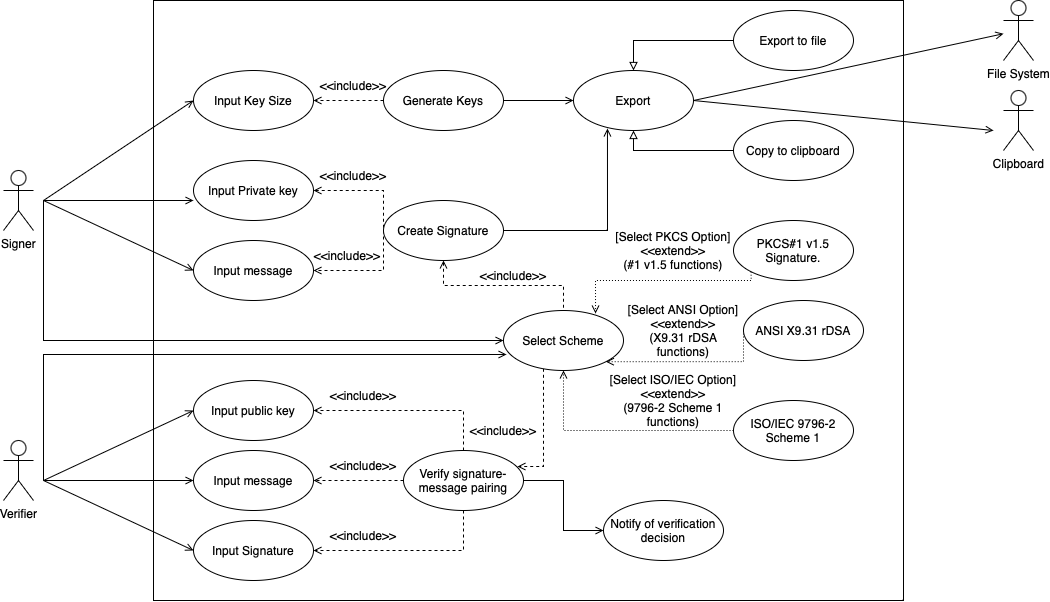
\includegraphics[scale=0.48]{poc_pictures/POC_USE-CASE.png}
    \caption{UML Use Case Diagram}
    \label{fig:uc}
\end{figure}

Please see Appendix Appendix B.1 for a full breakdown of relevant requirements (capturing essential behaviour), and a flow-of-events type description for figure \ref{fig:uc} representing completed UML use cases, derived from preceding user stories.



\section{A Horizontal Slice: Key Generation}
\subsection{Design}
\begin{figure}[H]
    \centering
    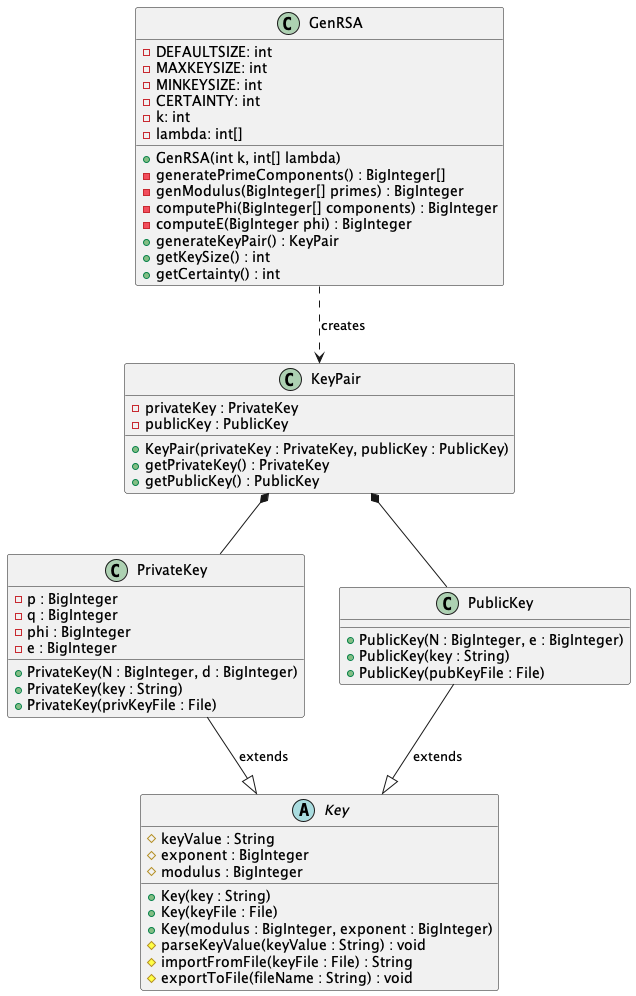
\includegraphics[scale=0.48]{poc_pictures/KeyGeneration.png}
    \caption{Key Generation Class Design}
    \label{fig:kg}
\end{figure}

Figure \ref{fig:kg} provides a conceptualised design view of the foundational GenRSA definition discussed in section  \ref{subSec:keygen} aiming to act as bridge to implementation. The process is broken down into smaller components corresponding to roles/entities supportive to the purpose of generating keys. 


\begin{table}[H]
    \centering
    \caption{GenRSA Design}
    \label{tab:actors_description}
    \begin{tabular}{|l|p{10cm}|}
    \hline
    \textbf{Class} & \textbf{Description} \\
    \hline
    KeyGenRSA & Central class responsible for generating the key pair by providing a method to fulfil the generation process. \\
    \hline
    Key & Abstract class that serves as a blueprint for the public and private keys, encapsulating the use of the modulus and an accompanying exponent with further the ability to import/export its content. \\
    \hline
    PrivateKey / PublicKey & These classes extend from Key, specialising it for private and public key functionalities respectively. \\
    \hline
    \end{tabular}
\end{table}



\subsection{Implementation}
My approach to key generation deviates from standard practices by offering customisable options, particularly in the number of prime factors forming the modulus. Unlike traditional methods that limit the number of primes to two, my code allows the user to specify any number of primes, each with different bit sizes. The modulus and, consequently, the RSA key, are computed based on this specification. This approach aligns with the generalised key generation process outlined in Section \ref{subSec:keygen}. It stems from the necessity to meet requirements for the considered security proofs for using a non-standard number of primes.

\begin{lstlisting}[caption=Initialisation of parametrisable Key Generation]
public GenRSA(int k, int[] lambda) throws IllegalArgumentException {
    if (lambda.length != k) {
      throw new IllegalArgumentException("Lambda array must have k elements.");
    }

    for (int bitLength : lambda) {
      keySize += bitLength;
    }

    this.k = k;
    this.lambda = lambda;
  }
 \end{lstlisting}
 
The suitability of Java's BigInteger class as discussed prior becomes evident from the outset. For example when the considering the foundational task for the proof of concept program: RSA Key Generation and more precisely the generation of the large primes required to encompass the modulus N.
Utilising the constructor BigInteger(int bitLength, int certainty, Random rnd), it is possible to generate probable prime numbers of some arbitrary value, provided a certainty level is indicated.
\begin{lstlisting}[caption=Parametrisable Prime Generation with BigInteger]
public BigInteger[] generatePrimeComponents() {
    BigInteger[] components = new BigInteger[k];
    for (int i = 0; i < k; i++) {
      components[i] = new BigInteger(lambda[i], this.certainty, new SecureRandom());
    }
    return components;
  }
\end{lstlisting}
As with any RSA implementation the first step is initialising the RSA primes. 
Due to the magnitude of the integers in question, attempting to factorise both p and q to establish their primality with absolute certainty is computationally impractical. Instead, BigInteger employs the Miller-Rabin primality test to assess the probability of primality based with the probability  \[ 1 - \frac{1}{2^{certainty}}\]
For a balance between security and practicality, a certainty value between 50-100 is typical. I chose the midpoint value as a practical compromise.

\begin{lstlisting}[caption=Key components]
  public BigInteger computePhi(BigInteger[] components) {
    BigInteger phi = BigInteger.ONE;
    for (BigInteger prime : components) {
      phi = phi.multiply(prime.subtract(ONE));
    }
    return phi;
  }
  
  public BigInteger computeE(BigInteger phi) {
    BigInteger e = new BigInteger(phi.bitLength(), new SecureRandom());
    while (e.compareTo(ONE) <= 0 || !phi.gcd(e).equals(ONE) || e.compareTo(phi) >= 0) {
      e = new BigInteger(phi.bitLength(), new SecureRandom());
    }
    return e;
  }
\end{lstlisting}
The public key, \( e \), should belong to the group \( (Z/ Z_{\phi})^{\times} \). To achieve this, a (positive) random \texttt{BigInteger} with the same number of bits as \( \phi \) is generated until a value from the group is identified. The \texttt{BigInteger} bitCount() method provides the means for doing this by returning the non-sign bit count of $\varphi$. 

The remaining computation in the attempt to obtain the private exponent d is straightforward with a naturally supported modInverse operation.
\begin{lstlisting}[caption=Java Implementation of Key Generation (\ref{subSec:keygen})]
  
  public KeyPair generateKeyPair() {
    BigInteger[] primes = this.generatePrimeComponents();
    BigInteger N = genModulus(primes);
    BigInteger phi = computePhi(primes);
    BigInteger e = computeE(phi);
    
    BigInteger d = e.modInverse(phi);
    PublicKey publicKey = new PublicKey(N, e);
    PrivateKey privateKey = new PrivateKey(N, primes, phi, e, d);

    return new KeyPair(publicKey, privateKey);
  }

\end{lstlisting}

\section{Design}
\textcolor{red} {For further design documentation see Appendix B.2.}

%\begin{landscape}
%\thispagestyle{lscape} % Apply the custom page style
\begin{figure}[H]
    \centering
    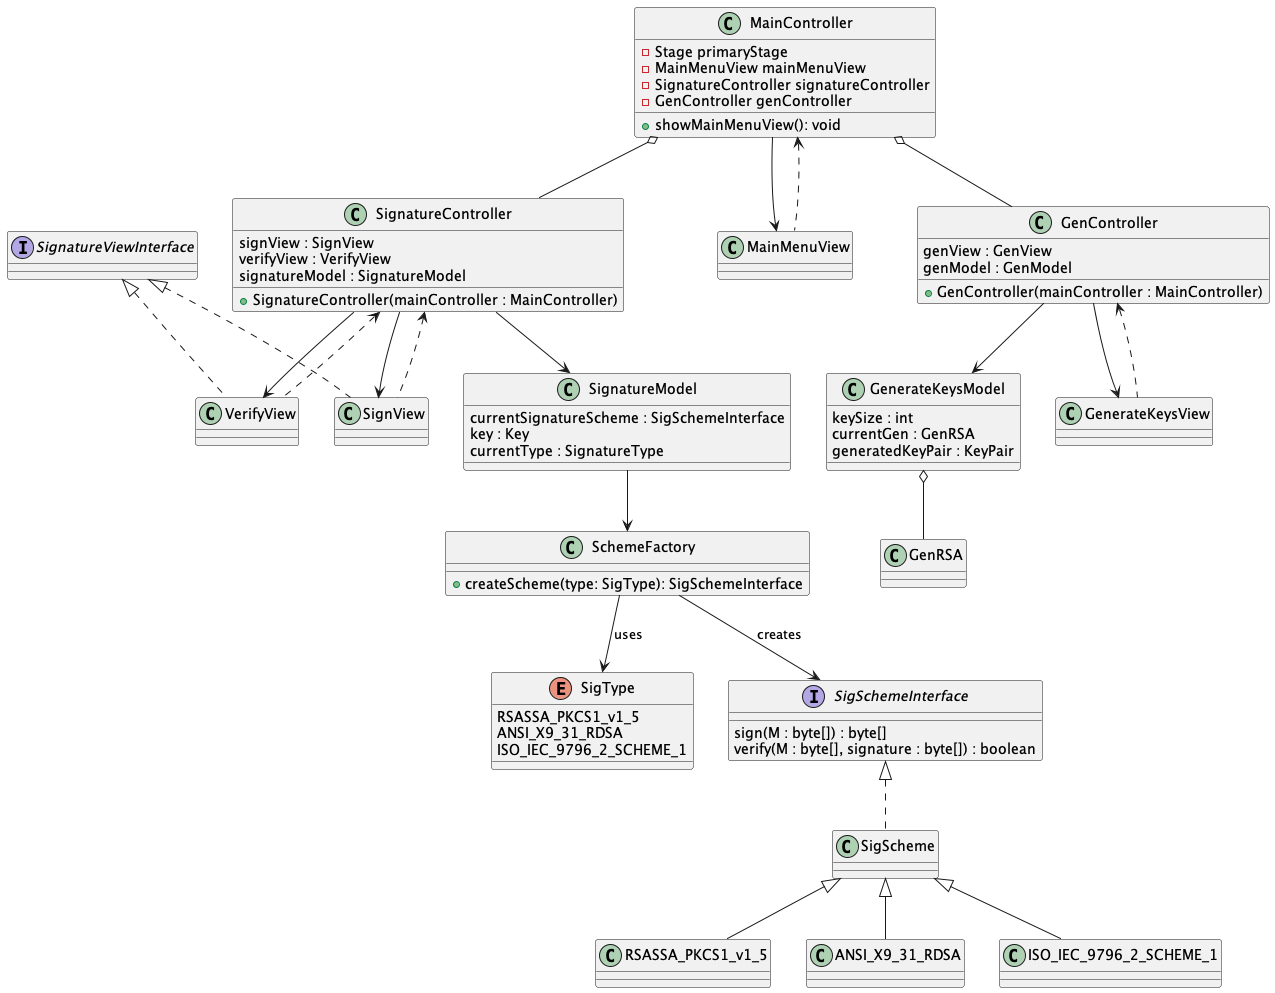
\includegraphics[width=\textwidth]{poc_pictures/POC.png}
    \caption{POC program Class Design}
    \label{fig:POCCLASSES}
\end{figure}
%\end{landscape}

\subsection{MVC pattern}
Figure \ref{fig:POCCLASSES} depicts the structure of classes to be used in the implementation of the PoC program.  There is a focus on separation of concerns following the Model-View-Controller (MVC) design pattern. In general terms it separates the application logic from the user interface and the control between the user interface and the application logic. At the heart of the design is the MainController, which orchestrates the application flow by responding to user actions and coordinating the display of different views. There are two applications of the MVC encapsulated within the MainController.

The first of these In support is the SignatureController, which manages the signature processes, linking the signature-related views (SignView and VerifyView) with the SignatureModel. The SignatureModel serves as software approximation of a real-world processes of the signing and verification processes. It encapsulates the cryptographic logic and relies on a SchemeFactory to instantiate a concrete signature scheme (as per user selection). The SignatureModel acts as an interface for the SignatureController into a tracked instance of a signature scheme (SigScheme). 

The signature-related views (SignView and VerifyView) render the contents of the SignatureModel updating presentation as needed if the model data changes.
The GenController mirrors the structure of the SignatureController but  is focused on generating cryptographic keys through the GenerateKeysModel which manages the GenRSA facilitated key creation.

\subsection{Observer pattern}
The UML diagram also hints at the observer pattern, a subset of MVC, with the Controllers acting as observers to the Views, which are the observables. When a user interacts with a View, such as initiating a signature generation request, the View notifies the SignatureController, which in turn invokes the necessary methods in both the View and the Model to fulfil the request. This decouples the user interface from the business logic, allowing for independent development and refinement of each component.

\subsection{Factory pattern}
The architecture of the signature program is based on the factory design pattern to enhance modularity and integration. This design choice is particularly useful when incorporating different RSA signature schemes like ANSI X9.31 and ISO/IEC 9796-2. In the program, each signature scheme is an implementation of a SigScheme class that follows a SigSchemeInterface. This interface is beneficial because it ensures that all signature schemes, despite their differences, conform to a standard set of operations such as key generation, hashing, and the signing and verification processes. These processes involve common cryptographic operations like encoding and converting between integers and octet strings.

The SchemeFactory class abstracts the complexity of creating instances of these signature schemes. This abstraction allows the SignatureModel to reference and use different signature schemes without being tied to their concrete implementations. Essentially, the SchemeFactory takes care of the details behind object creation, allowing the SignatureModel to work with a higher level of abstraction and to interact with any signature scheme through a common interface.

This approach helps keep the SignatureModel clean and focused on its primary responsibilities rather than the nuances of how each signature scheme is instantiated. The result is a flexible and easily maintainable codebase that can readily accommodate new signature schemes as they become relevant, without the need to overhaul the existing system.


\section{Implementation: Overview}

This section presents a high level overview of the main functionality of the overall program.
\begin{comment}
\textcolor{red} {For lower level detail related to implementation of the schemes, see Appendix B.3.}
\end{comment}

The application contains four main windows:
\begin{enumerate}
\item Main Menu - The starting point of the application. Serves as a portal to a selected key/signature functionality. 
\item Key Generation - Serves as the means for generating the RSA Keys compatible with signature processes in the application. 
\item Signature Creation - Serves as the means for generating signatures of one of the considered deterministic types.
\item Signature Verification - Serves as the means for verifying whether an application compatible signature is valid on a selected message of the users choice.
\end{enumerate}



\subsection{Main Menu}

\begin{figure}[H]
    \centering
    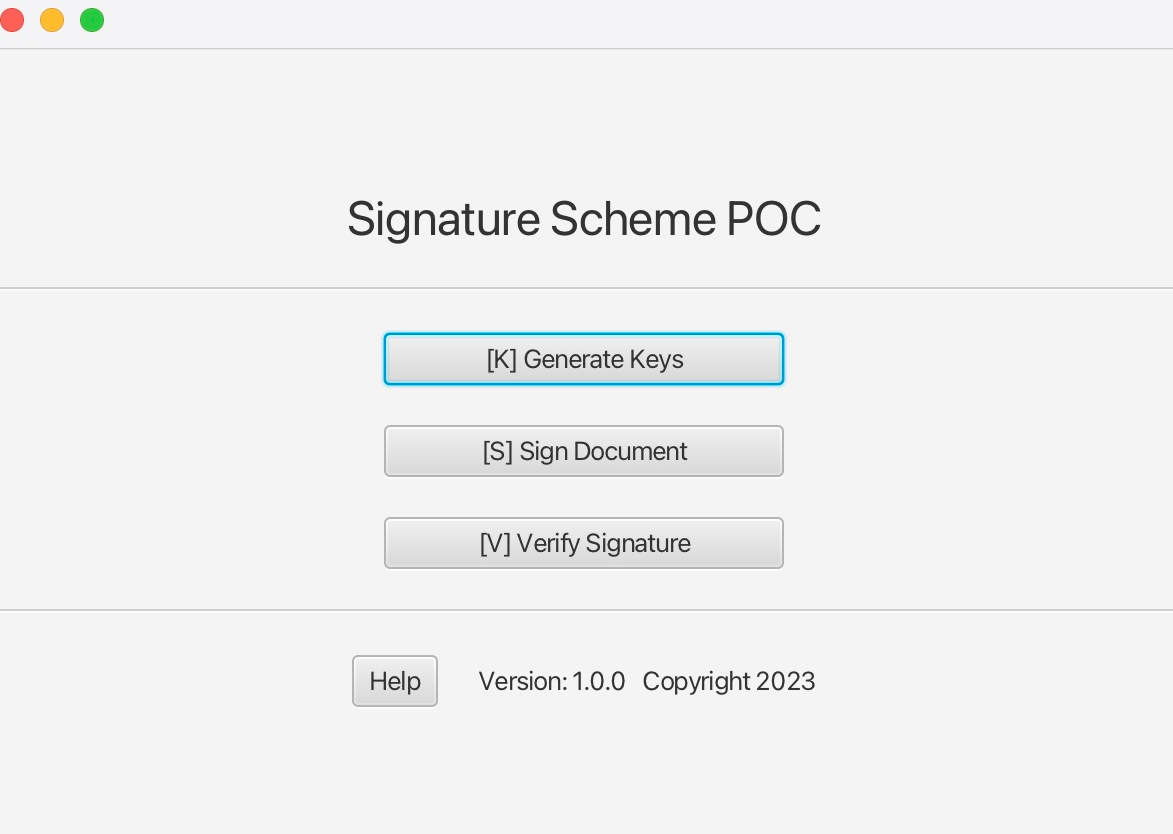
\includegraphics[scale=0.3]{poc_pictures/mainMenu.png}
    \caption{Main Menu}
\end{figure}
The main menu screen of the application presents a straightforward and functional layout, serving as the gateway to its core features via menu buttons. Its design is realised through an FXML layout file, which defines the graphical user interface elements such as buttons. Each button on the main menu is associated with a specific functionality and is observable by the virtue of its MainMenu domain object class. For example, the "Generate Keys" button is linked to the following method contained in the class:
\begin{lstlisting}[caption=Mechanism for registering observers]
@FXML private Button generateKeysButton;

void addGenerateKeysObserver(EventHandler<ActionEvent> observer) {
  generateKeysButton.setOnAction(observer);
}
\end{lstlisting}
The above is the mechanism that enables the MainController to register observers and in turn observe the main menu. The MainController underpins the main menu, setting the primary stage of the application and showing the MainMenuView as the initial scene.


\begin{lstlisting}[caption=MainController registering an observer to be notified on selection of key generation button]
void showMainMenuView() {
  FXMLLoader loader = new FXMLLoader(getClass().getResource("/MainMenuView.fxml"));
  Parent root = loader.load();
  mainMenuView = loader.getController();
  primaryStage.setScene(new Scene(root));
  primaryStage.show();

  mainMenuView.addGenerateKeysObserver(new GenerateKeysButtonObserver());
  // ...additional observers for other buttons
}
\end{lstlisting}
On launch the MainController registers observers on the observable components of the main menu screen. When a user interacts with the interface by clicking a button, the associated observer is notified, and its effects are triggered. For example, the GenerateKeysButtonObserver will instantiate a new GenController which takes over and presents the key generation view to the user. 


\begin{lstlisting}[caption=Implementation of an observer]
public class MainController {
  private Stage primaryStage;
  private GenController genController;
  private SignatureController signatureController;

  class GenerateKeysButtonObserver implements EventHandler<ActionEvent> {

    @Override
    public void handle(ActionEvent event) {
      genController = new GenController(MainController.this);
      genController.showGenView(primaryStage);
    }
  }
\end{lstlisting}
The equivalent patterns is followed for all other components in the design of the program. From this point we assume its usage.
\subsection{Key Generation}
\begin{figure}[h]
    \centering % Center the images
    
    % First image in a minipage
    \begin{minipage}{0.49\textwidth}
        \centering
        \fbox{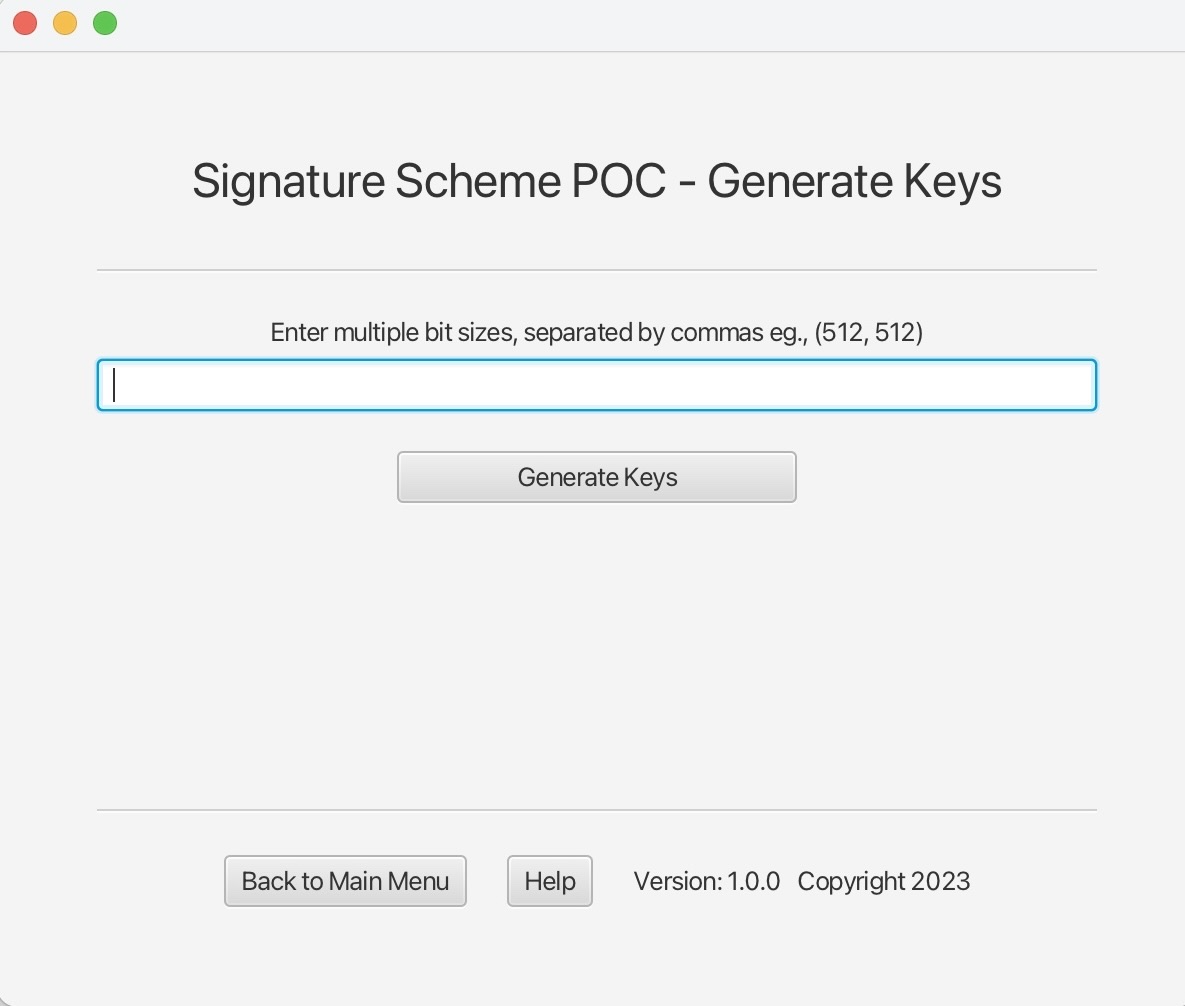
\includegraphics[width=\textwidth]{poc_pictures/keyGen.png}} % Adding border here
        \caption{Key Generation Screen}
        \label{fig:image1}
    \end{minipage}
    \hfill % Add some space between the images
    % Second image in a minipage
    \begin{minipage}{0.49\textwidth}
        \centering
        \fbox{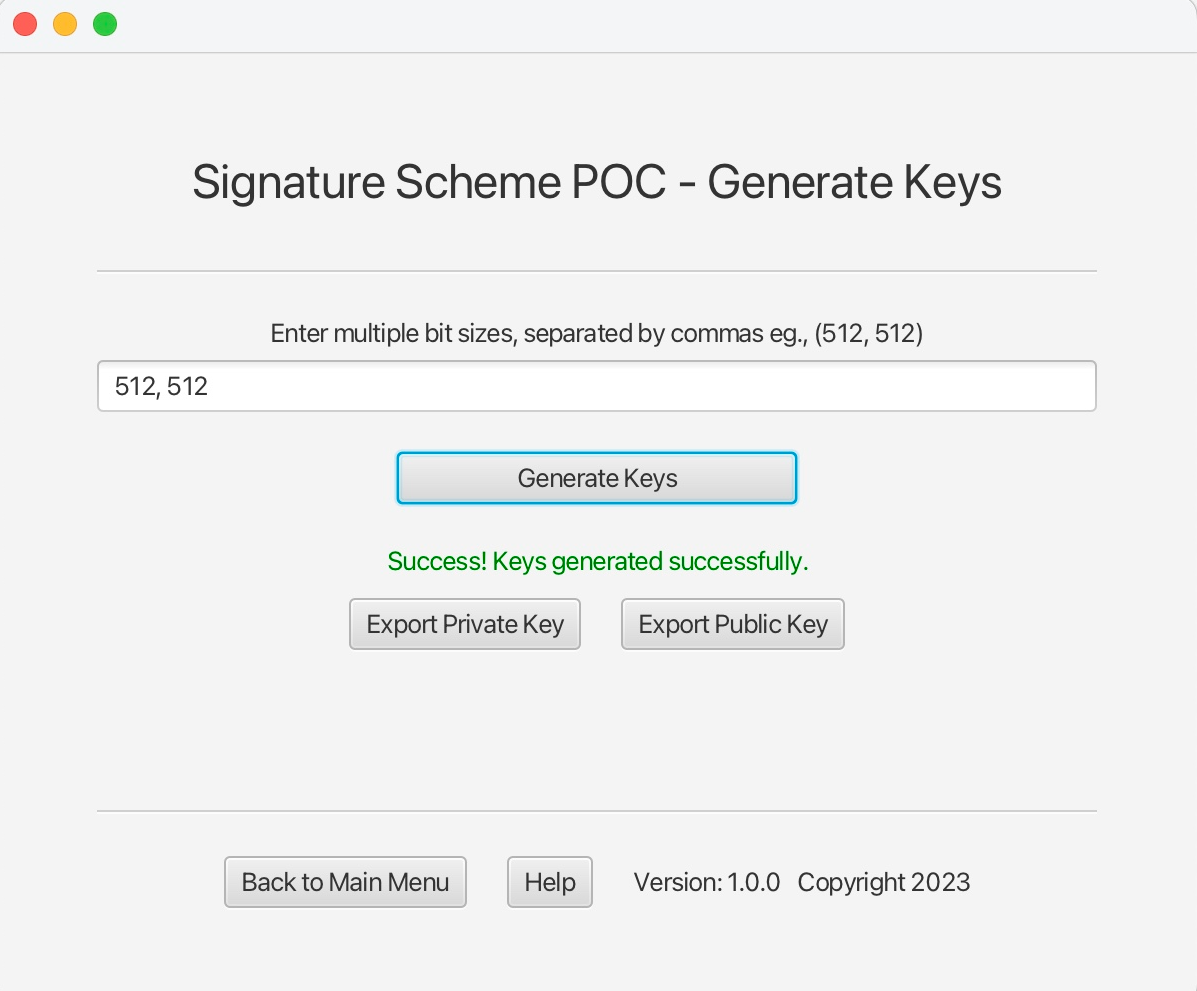
\includegraphics[width=\textwidth]{poc_pictures/keyGenSuccess.png}} % Adding border here
        \caption{Key Generation Success}
        \label{fig:image2}
    \end{minipage}
\end{figure}
The key generation screen serves as a specialised portal within the application, where users are invited to specify parameters for cryptographic key creation. The screen features an input box for key size parameters and a "Generate Keys" button, which sets the key generation process in motion.

Behind the scenes, the GenController class orchestrates the user interactions on this screen. It waits to be notified by the view of activation of the "Generate Keys" button, which triggers a series of operations. Initially, the input from the user is subjected to a validation process. This ensures that the provided bit sizes are in an acceptable format and within the operational range for key generation. If the input is incorrect or the key generation encounters an issue, then an alert is displayed with an appropriate message to the user. 

Upon successful validation, the GenModel is engaged to carry out the key generation. It is instructed with the parameters provided by the user, after which it proceeds to generate the RSA key pair. Once the keys are generated, the application offers the facility to export them. Additionally, the screen includes a navigational aid in the "Back to Main Menu" button that gracefully transitions the user back to the main menu of the application.


\subsection{Signature Generation}
\begin{figure}[H]
    \centering % Center the images
    
    % First image in a minipage
    \begin{minipage}{0.49\textwidth}
        \centering
        \fbox{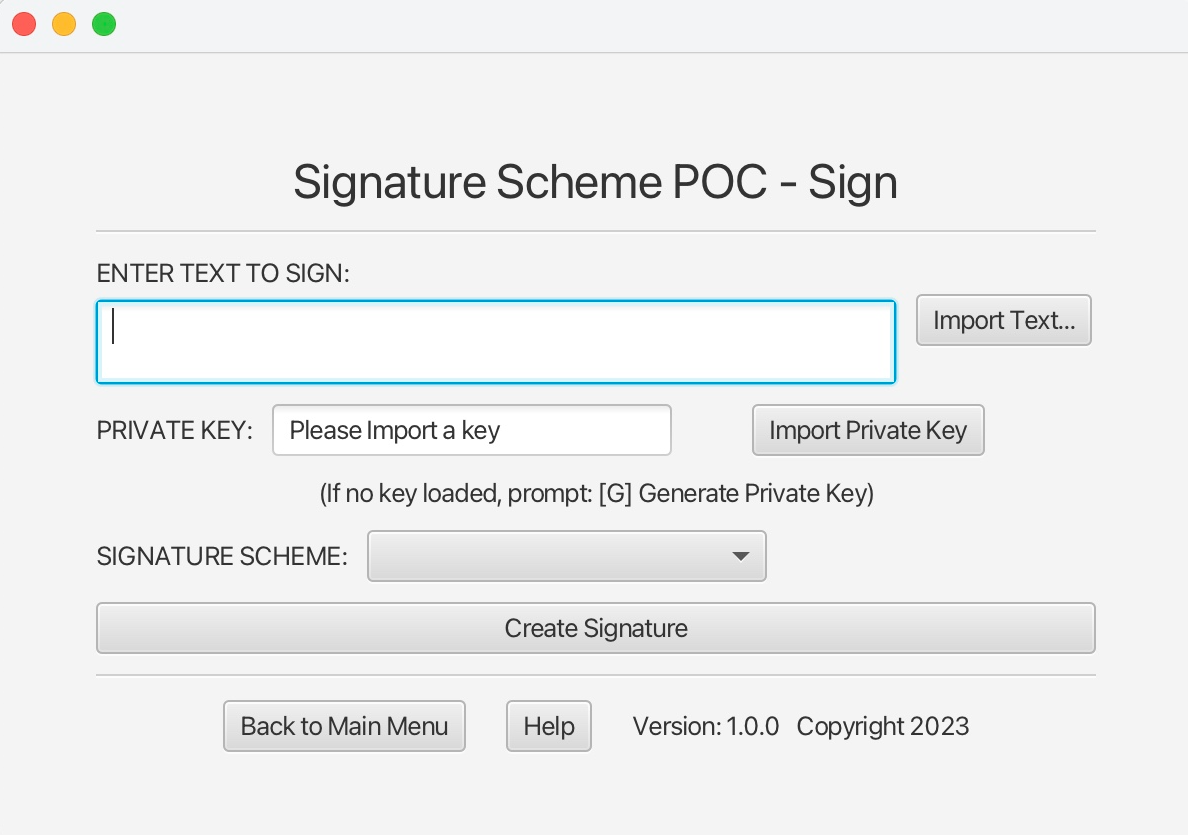
\includegraphics[width=\textwidth]{poc_pictures/sign.png}} % Adding border here
        \caption{Initial Signature Creation Screen}
        \label{fig:image1}
    \end{minipage}
    \hfill % Add some space between the images
    % Second image in a minipage
    \begin{minipage}{0.49\textwidth}
        \centering
        \fbox{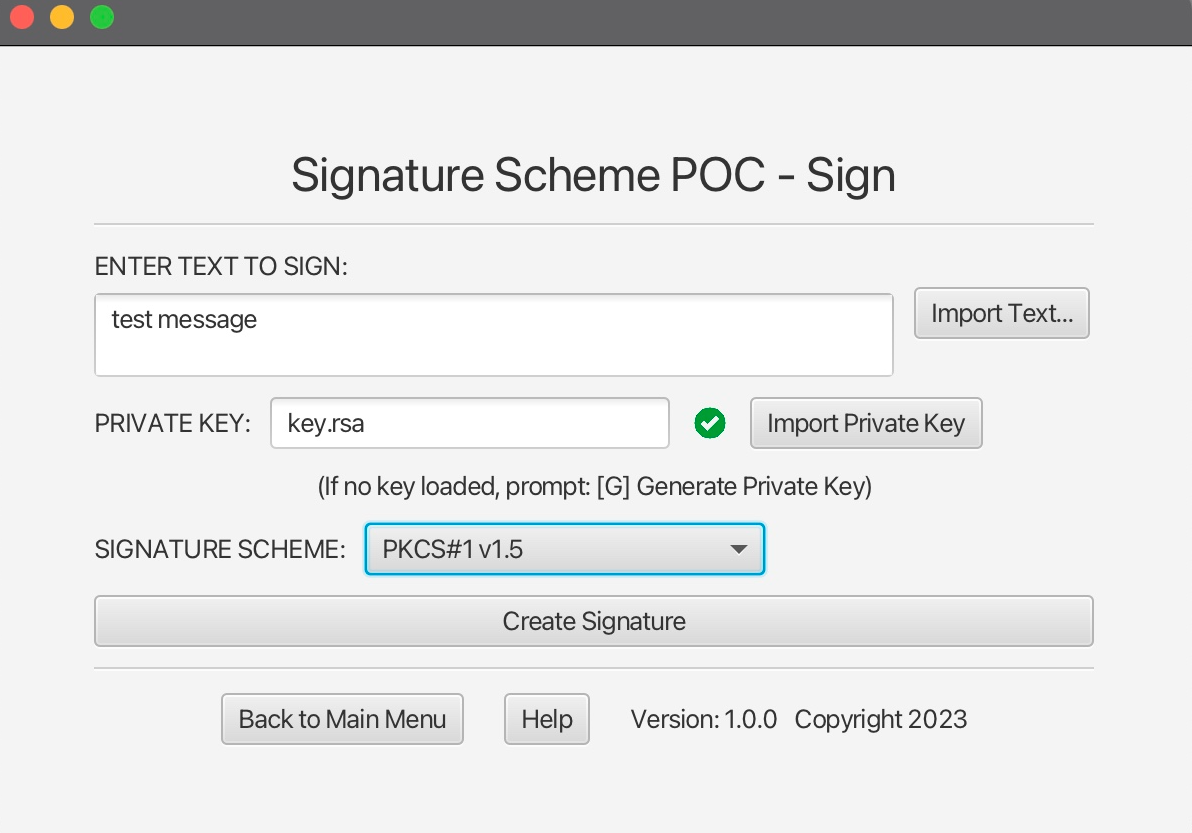
\includegraphics[width=\textwidth]{poc_pictures/signInput.png}} % Adding border here
        \caption{Signature Creation Screen with all inputs}
        \label{fig:image2}
    \end{minipage}
\end{figure}


The signature creation screen acts as a dedicated hub within the application, designed for users to engage in the signing of documents. This screen is organised with an input field for users to either type or import the text that they wish to sign. In the backdrop, the SignatureController class waits to be notified of interaction with the import button. Upon successful validation it updates the screen with a checkmark indicator that provides visual confirmation that the text was successfully imported. Adjacent to this is the private key import section, which also confirms successful key loading with a checkmark. 

The interface also includes a dropdown menu labeled giving users the option to select the desired signature scheme  to be applied. 
Upon selection of the "Create Signature" button, a chain of validation and execution steps are executed. The SignatureController first verifies that the text input and private key are valid and present. Should any discrepancies arise during this stage, the interface promptly presents an alert, informing the user of the necessary corrective measures.

\begin{figure}[H]
    \centering
    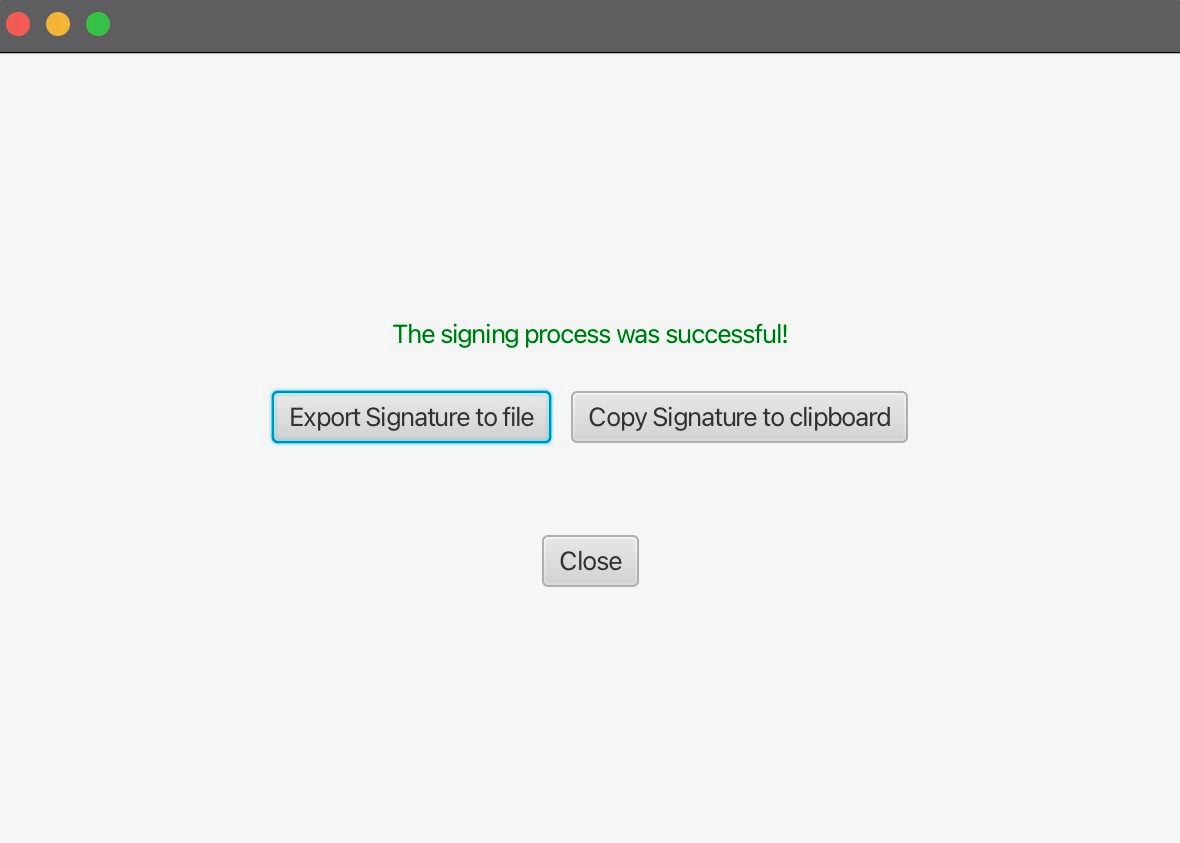
\includegraphics[width=0.6\textwidth]{poc_pictures/signSuccess.png}
    \caption{Signature Creation Success}
\end{figure}

Once the preliminary checks are satisfied, the SignatureModel takes over to perform the cryptographic operations, applying the chosen signature scheme to the text with the private key to generate a digital signature. Following this, the screen transitions to present the outcome of the signing process. If the process is successful, users are presented with a dialogue or a notification area within the interface, confirming the success and providing options to export the signature to a file or copy it to the clipboard.

\begin{figure}[h]
    \centering % Center the images
    
    % First image in a minipage
    \begin{minipage}{0.49\textwidth}
        \centering
        \fbox{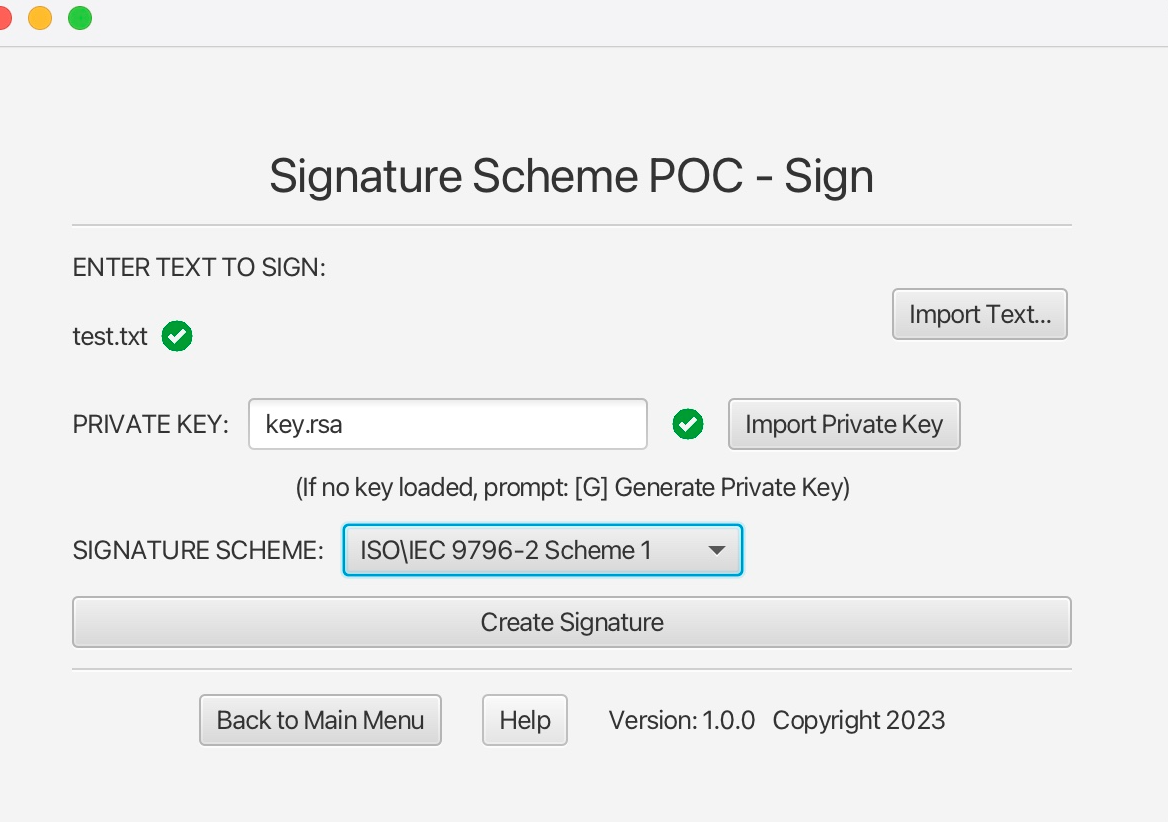
\includegraphics[width=\textwidth]{poc_pictures/isoSelected.png}} % Adding border here
        \caption{Signature Creation with ISO scheme selected}
        \label{fig:image1}
    \end{minipage}
    \hfill % Add some space between the images
    % Second image in a minipage
    \begin{minipage}{0.49\textwidth}
        \centering
        \fbox{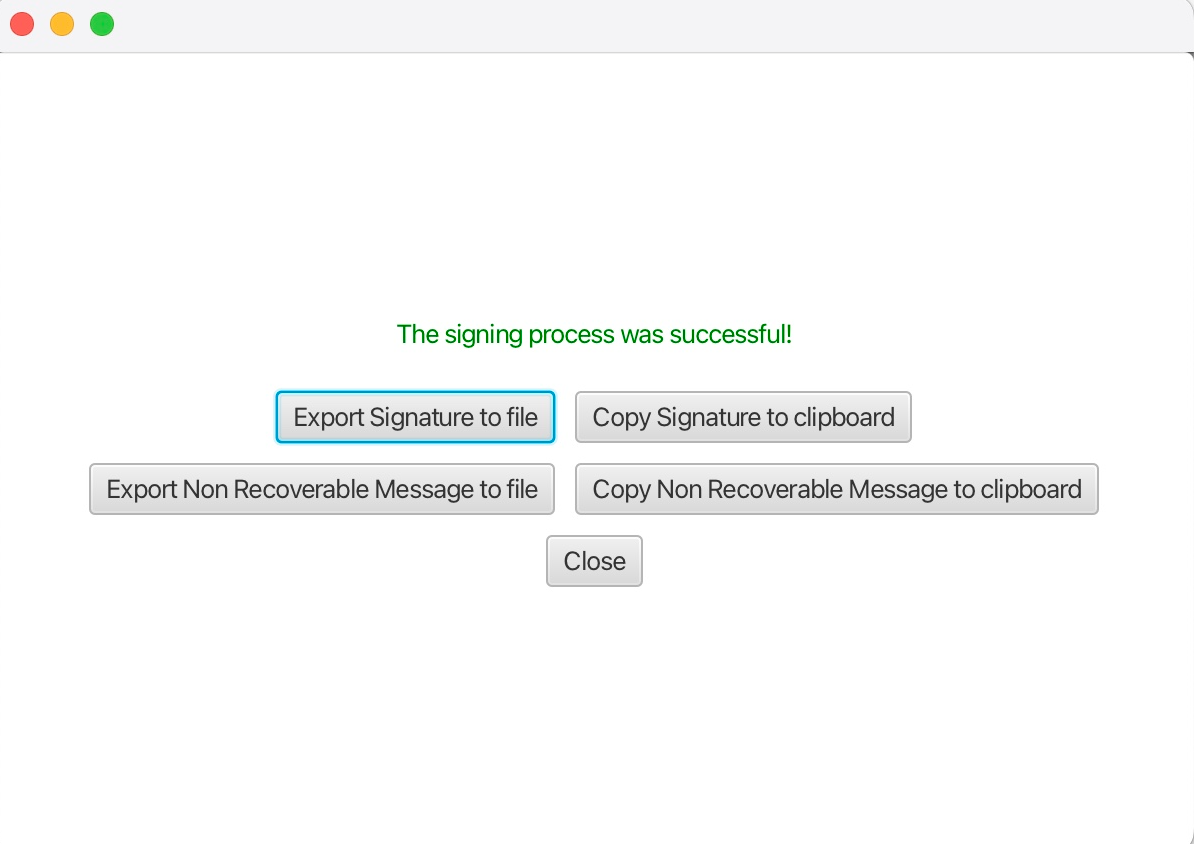
\includegraphics[width=\textwidth]{poc_pictures/signRecovery.png}} % Adding border here
        \caption{Signature Creation Success with message recovery options}
        \label{fig:image2}
    \end{minipage}
\end{figure}

When using a signature scheme that supports message recovery, such as ISO \slash IEC 9796-2 Scheme 1, and a part of the document is non-recoverable (cannot be reconstructed solely from the signature), the notification panel presents further relevant options for exporting.
Finally, users can navigate back to the main menu at any point through the BackToMainMenu option, maintaining a smooth user experience throughout the application.

\subsection{Signature Verification}

\begin{figure}[H]
    \centering % Center the images
    
    % First image in a minipage
    \begin{minipage}{0.49\textwidth}
        \centering
        \fbox{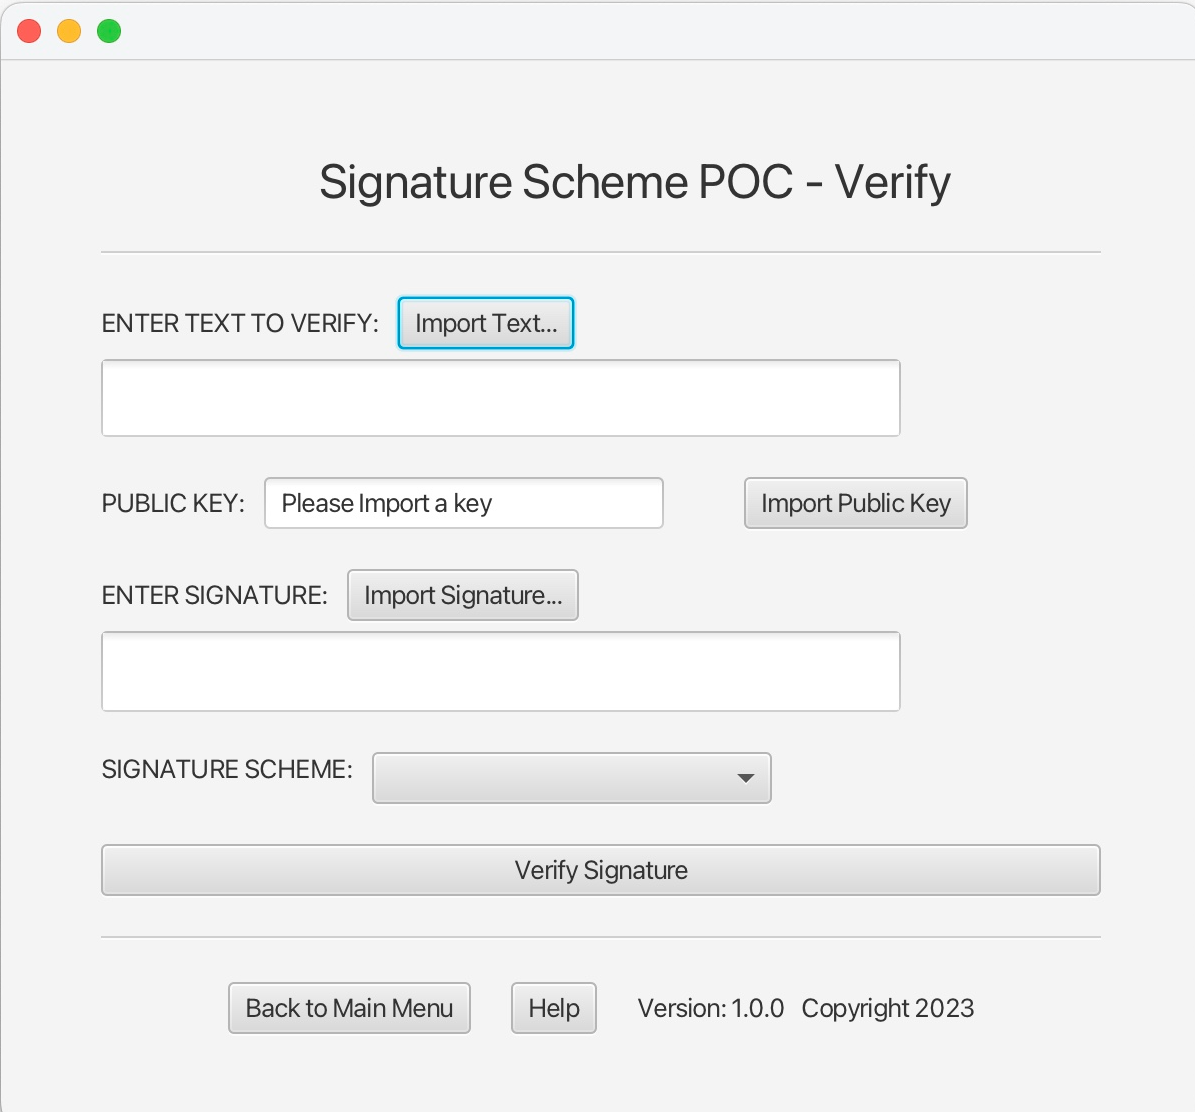
\includegraphics[width=\textwidth]{poc_pictures/verify.png}} % Adding border here
        \caption{Initial Verification view Screen}
        \label{fig:image1}
    \end{minipage}
    \hfill % Add some space between the images
    % Second image in a minipage
    \begin{minipage}{0.49\textwidth}
        \centering
        \fbox{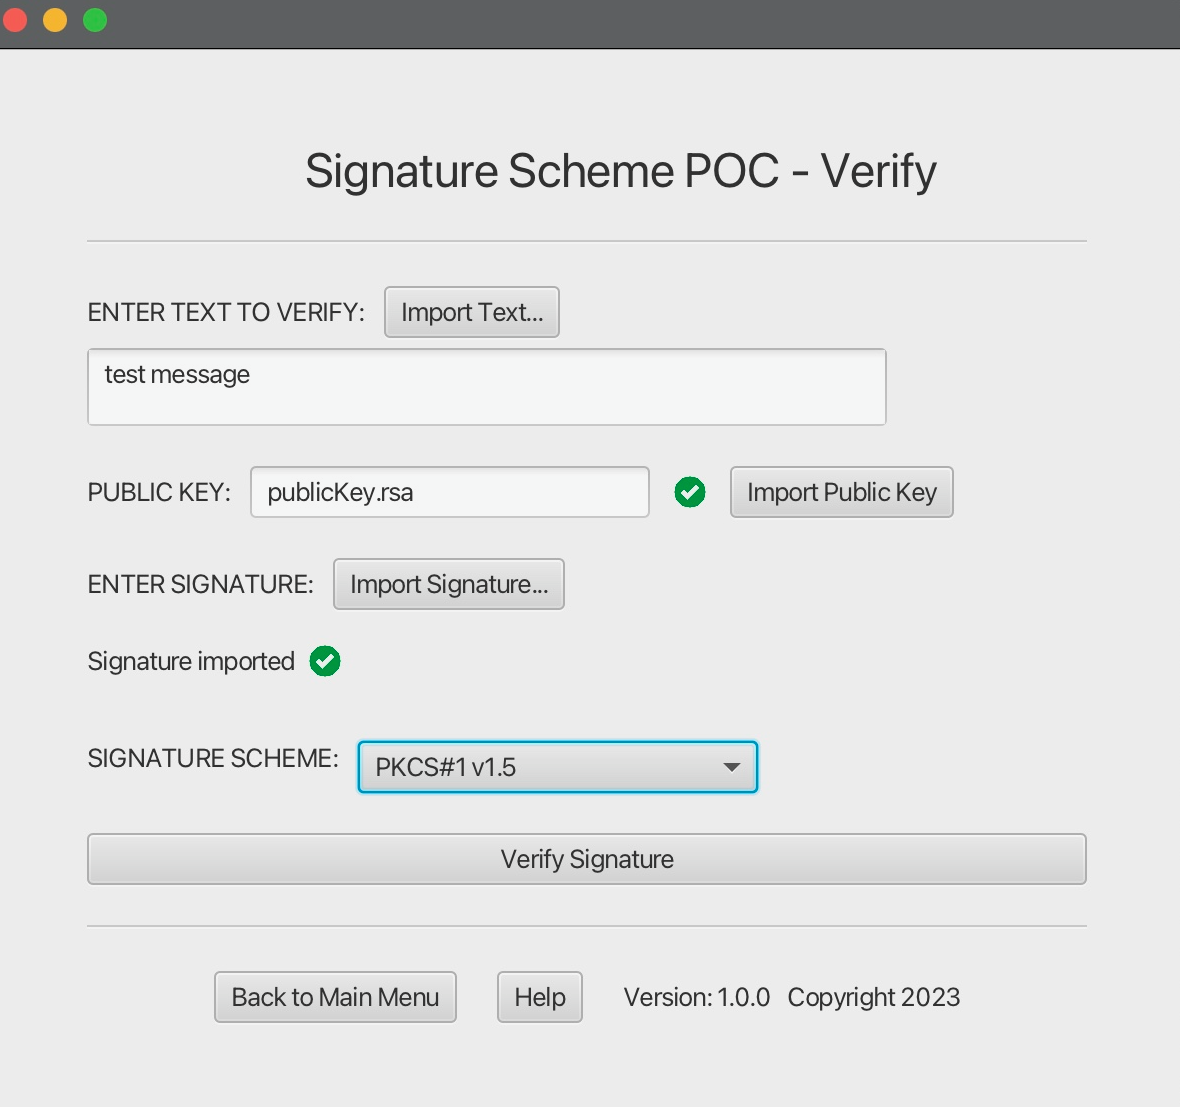
\includegraphics[width=\textwidth]{poc_pictures/verifyInput.png}} % Adding border here
        \caption{Verification Screen with all inputs entered}
        \label{fig:image2}
    \end{minipage}
\end{figure}

The signature verification screen acts as a dedicated hub within the application, designed for users to engage in the verification of signatures. This screen is organised with an input field for users to either type or import the text related to the signature they wish to verify. In the event of interaction with the import button, the screen updates with a checkmark indicator that provides visual confirmation that the text was successfully imported. Similar goes for the distinct public key and signature import sections. The process echoes mechanism discussed previously as per the signature creation screen.

Below these fields, a dropdown menu invites users to select the signature scheme applied when the signature was created, ensuring the correct verification method is used.
Upon selection of the "Verify Signature" button, a chain of validation and execution steps are executed. The SignatureController first verifies that the text input, public key and signature are valid and present. Should any discrepancies arise during this stage, the interface promptly presents an alert, informing the user of the necessary corrective measures.

\begin{figure}[H]
    \centering
    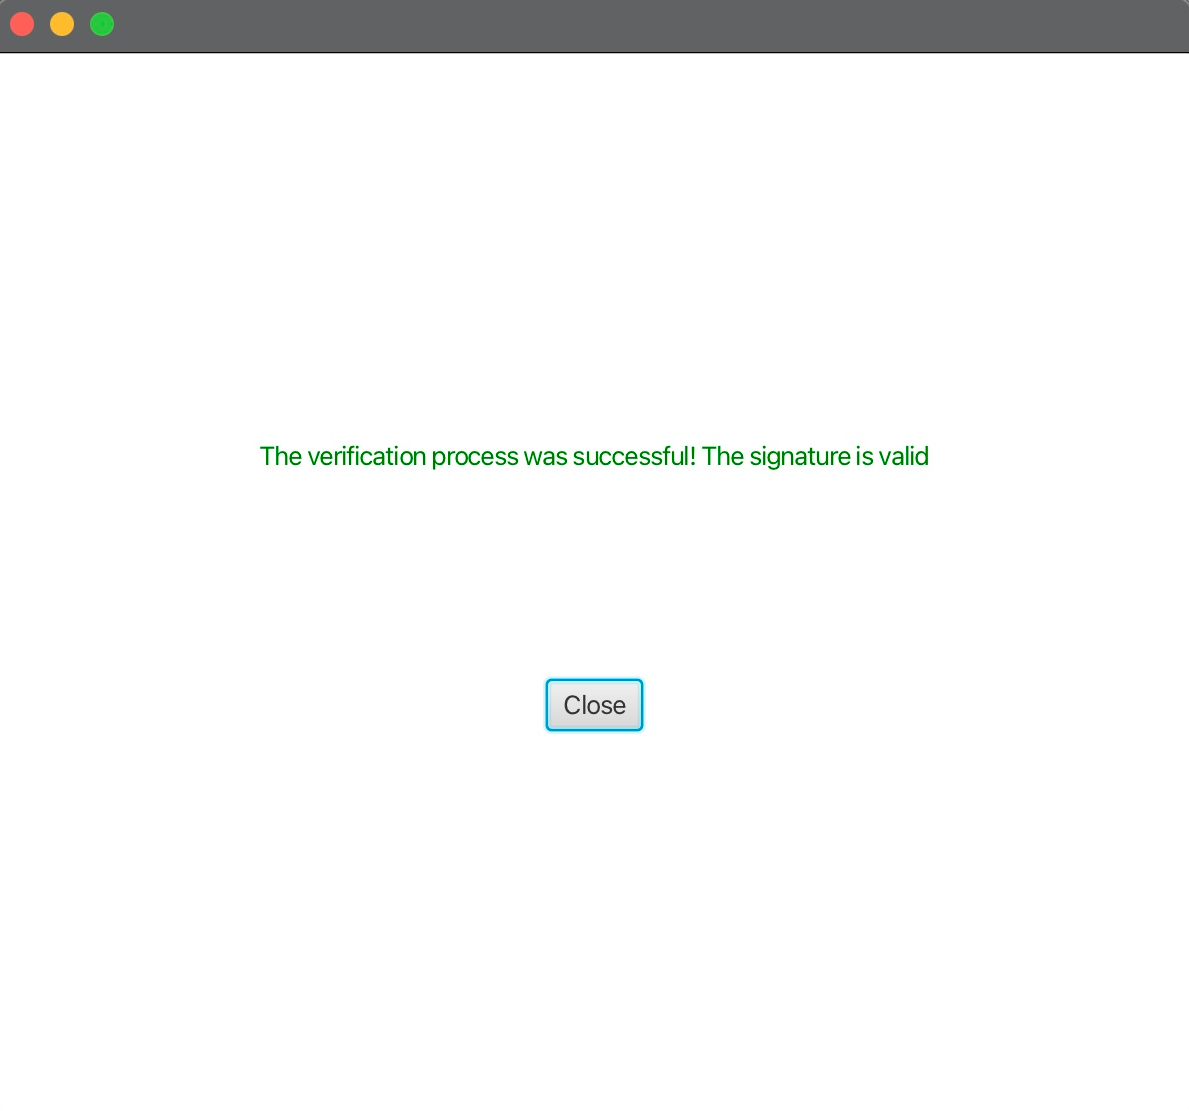
\includegraphics[width=0.55\textwidth]{poc_pictures/verifyTrue.png}
    \caption{Verification Success Pop-up}
\end{figure}

Once the preliminary checks are satisfied, the SignatureModel takes over to perform the cryptographic operations, comparing the provided signature against the message with public key using the selected signature scheme to generate a verification result. Following this, the screen transitions to present the outcome of the verification process. 


\begin{figure}[h]
    \centering % Center the images
    
    % First image in a minipage
    \begin{minipage}{0.49\textwidth}
        \centering
        \fbox{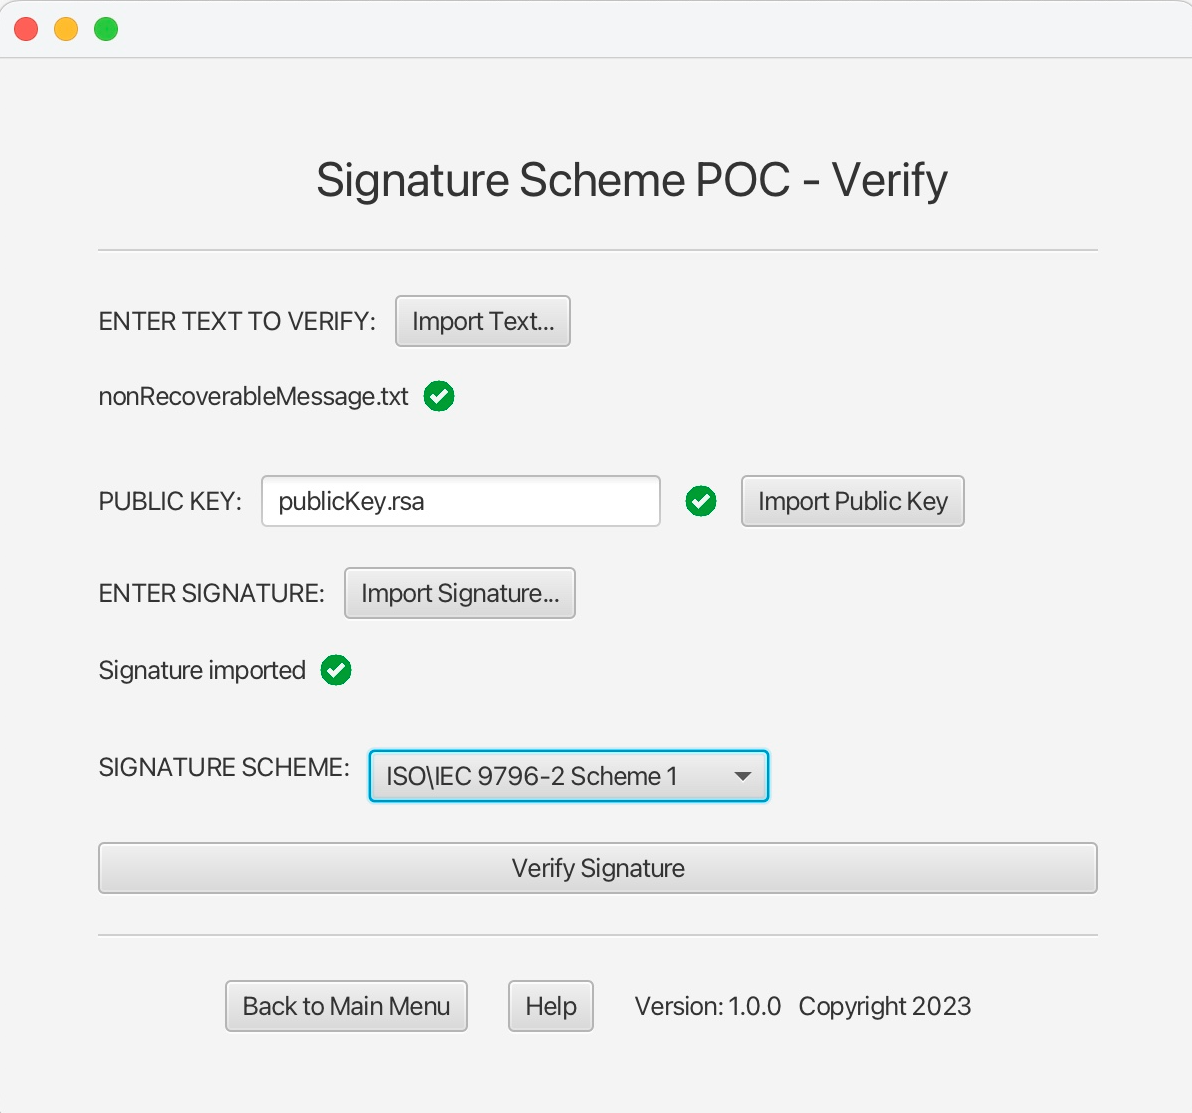
\includegraphics[width=\textwidth]{poc_pictures/verifyISO.png}} % Adding border here
        \caption{Signature verification with ISO scheme selected}
        \label{fig:image1}
    \end{minipage}
    \hfill % Add some space between the images
    % Second image in a minipage
    \begin{minipage}{0.49\textwidth}
        \centering
        \fbox{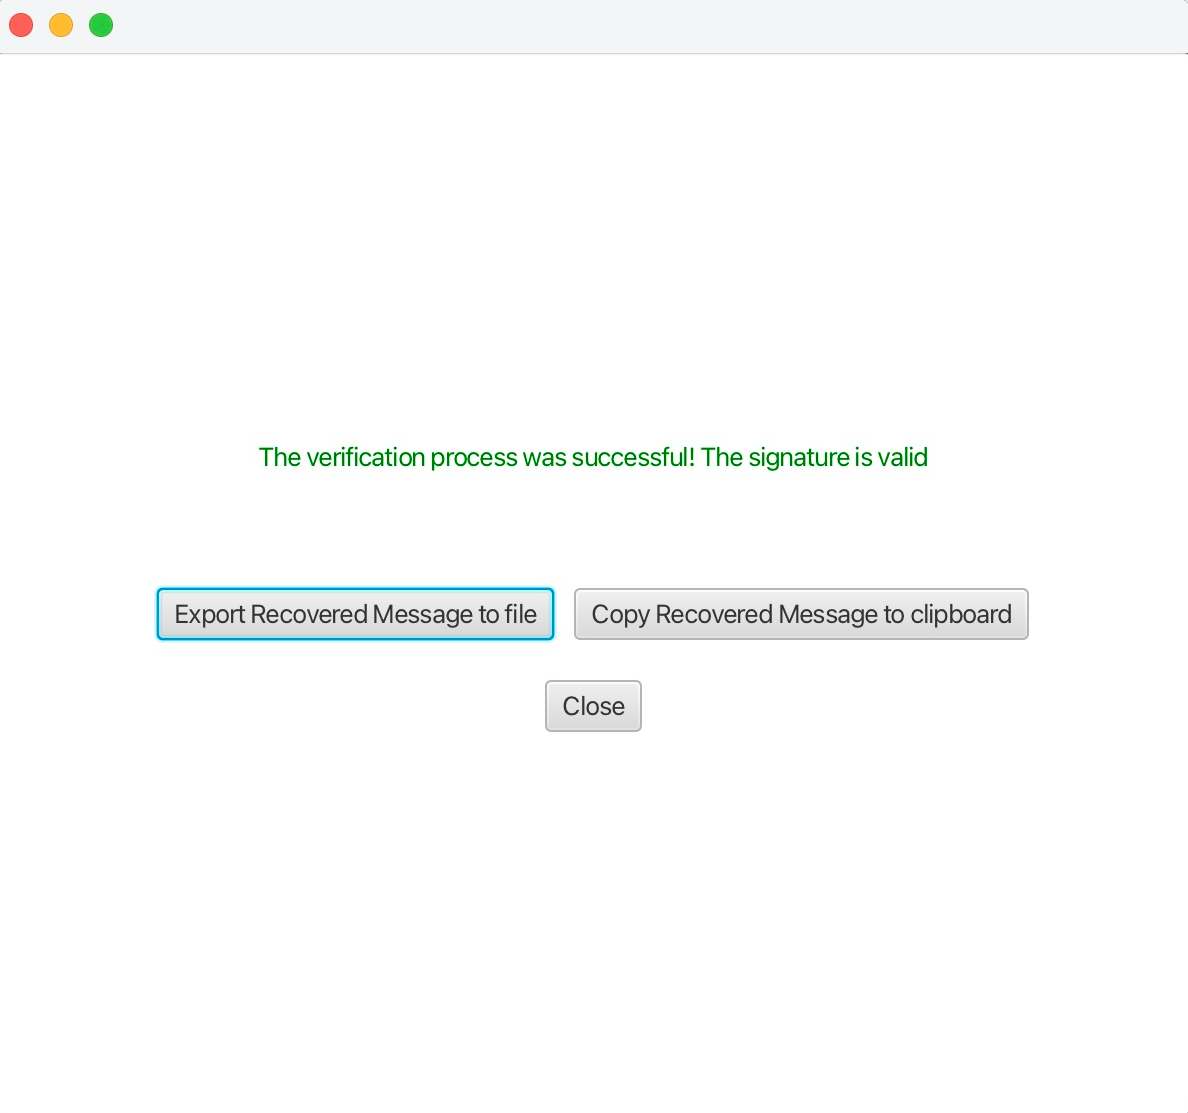
\includegraphics[width=\textwidth]{poc_pictures/verifyRecovery.png}} % Adding border here
        \caption{Signature Verification Success with message recovery options}
        \label{fig:image2}
    \end{minipage}
\end{figure}

When using a message recovery-type signature scheme like ISO\slash IEC 9796-2 Scheme 1, successful signature verification allows for the recovered message to be exported. Notably, verifying an ISO/IEC 9796-2 Scheme 1 signature does not require the original text input in cases of full message recovery. This is because the goal of verification here is to extract the complete message initially fed into the signature generation process from the signature itself.

\textcolor{red} {For insight into the testing process see Appendix B.3 for more details.}

\section{Implementation: An Extensible Signature Scheme framework}
Having explored the theoretical underpinnings and practical applications of digital signature schemes, we now transition to a more technical focus of how signature schemes can be concretely implemented with a generalised framework.

The foundation of this is provided by SigSchemeInterface, an interface that outlines the essential functionalities required for any digital signature scheme. This interface serves as a contract for implementing classes, ensuring that fundamental operations such as signing, verifying, and data conversion between different formats are standardised and consistent.

\begin{lstlisting}[caption=SigSchemeInterface Interface code] 
public interface SigSchemeInterface {

  byte[] sign(byte[] M) throws SignatureException, DataFormatException;

  boolean verify(byte[] data, byte[] signature) throws SignatureException, DataFormatException;

  BigInteger OS2IP(byte[] EM);

  byte[] I2OSP(BigInteger m) throws IllegalArgumentException;

  BigInteger RSASP1(BigInteger m);

  BigInteger RSAVP1(BigInteger s);
}
 \end{lstlisting}

Signing a message m (sign(m)) works as follows:
\begin{enumerate}
\item Encode the message: encodeMessage(m).

\item Convert the message to representative integer form: OS2IP(m).

\item Using a private key sk, calculate the signature representative s using RSA: RSASP1(sk, m).

\item Convert the signature (integer) representative back to a byte string: I2OSP(s).
\end{enumerate}

Verification is the reverse, adapted accordingly. Given a signature s (verify(s)):

\begin{enumerate}
\item Convert s into an integer representative: OS2IP(s).

\item Using public key vk, calculate the message representative m: RSAVP1(vk, s)

\item Convert m to a byte string: I2OSP(m).

\item Verify the byte string using verifyMessage.
\end{enumerate}

We also note two further methods: 'encodeMessage', an algorithm to format data before performing a cryptographic signing operation on its integer representation, and 'verifyMessage', an algorithm that verifies the signature after a cryptographic verification operation has been performed on its integer representation. 
 
Building upon the SigSchemeInterface, the abstract class SigScheme is introduced as a concrete implementation of the Interface for implementing RSA-based signature schemes. This class provides standardised implementations of the interface's methods and 
includes additional functionality specific to RSA operations. It encapsulates key components like the RSA modulus, exponent, and message digest, contributing to a modular and extensible design suitable for various RSA-based signature schemes.

\begin{lstlisting}[caption=Implementation of RSA primitives]

  /**
   * Converts a BigInteger to an octet string of length emLen is the byte length of the RSA modulus.
   */
  public byte[] I2OSP(BigInteger m) throws IllegalArgumentException {
    return ByteArrayConverter.toFixedLengthByteArray(m, this.emLen);
  }

  /**
   * Calculates the RSA signature of a given message representative by raising it to the power of
   * the private exponent as outlined by the RSA algorithm.
   */
  public BigInteger RSASP1(BigInteger m) {
    BigInteger s = m.modPow(this.exponent, this.modulus);
    return s;
  }

  /**
   * Facilitates the verification of RSA signature by raising it to the power of the public exponent
   * as outlined by the RSA algorithm.
   */
  public BigInteger RSAVP1(BigInteger s) {
    return this.RSASP1(s);
  }

}
 \end{lstlisting}
We note that the implementation of RSAVP1 re-uses RSASP1. This design choice is viable because the exponent field in the SigScheme class is generic and can represent either the public or private exponent, depending on the type of key the scheme is instantiated with. This reuse simplifies the code and centralises the modular exponentiation logic in one place.
\newline

\begin{lstlisting}[caption=]
  public BigInteger OS2IP(byte[] EM) {
    return new BigInteger(1, EM);
  }
 \end{lstlisting}
For octet string to integer conversion, the BigInteger(int signum, byte[] magnitude) constructor provides a concise application of the concept succinctly converting the byte array that represents an octet string. The signum is set to 1 (since messages are non-negative) and the byte array of the message acts as the magnitude. The end result is a BigInteger representation of the message, which can then be used in RSA signing or verification processes.

 
The implementation of signing and verification processes essentially mirrors the pseudocode from the start of the section. 

\begin{lstlisting}[caption=Signature Scheme specialisation methods]
  // Abstract method to be implemented by derived classes for encoding
  protected abstract byte[] encodeMessage(byte[] M) throws DataFormatException;

  public boolean verifyMessage(byte[] M, byte[] S)
      throws DataFormatException {
    BigInteger s = OS2IP(S);
    BigInteger m = RSAVP1(s);
    byte[] EM;
    try {
      EM = I2OSP(m);
    } catch (IllegalArgumentException e) {
      return false;
    }

    byte[] EMprime = encodeMessage(M);

    return Arrays.equals(EM, EMprime);
  }
 \end{lstlisting}
 
The SigScheme class provides two further methods as compared to the interface with encodeMessage and verifyMessage. The encodeMessage method is left abstract because the encoding of messages is essentially what distinguishes different signature schemes. On the other hand, verifyMessage has a standardised implementation because, in many cases, it simply reverses the signing process. Since the core logic of this reversal often follows a standard procedure that is largely independent of the specifics of the message encoding, it is feasible to provide a standardised implementation for verifyMessage within the SigScheme class.

\textbf{Message Recovery}

Message recovery schemes, such as ISO/IEC 9796-2 Scheme 1, represent a special case, thereby challenging the notion of standardised implementations for key methods like sign and verifyMessage.
\begin{lstlisting}[caption=Implementation changes for Message Recovery Schemes]
public abstract class SigScheme implements SigSchemeInterface {

  byte[] nonRecoverableM;

  byte[] recoverableM;
}
public class ISO_IEC_9796_2_SCHEME_1 extends SigScheme {
  @Override
  public byte[] sign(byte[] M) throws DataFormatException {
    byte[] S = super.sign(M);
    // Extract m2 from the original message M using the computed m2's length
    if (m2Len > 0) {
      nonRecoverableM = Arrays.copyOfRange(M, m1Len - m2Len, m1Len);
    }
    return S;
  }
}
 \end{lstlisting}
The sign method for these schemes needs to be able to set the non recoverable message field of the class, to allow the respective portion message to be returned to the user, as part of the conclusion to the signature creation process. Hence, the ISO/IEC 9796-2 Scheme 1 class includes an overridden implementation of sign modified accordingly to account for this.

Along these same lines the verifyMessage method which we omit for brevity has to incorporate logic related to the separation of the message into recoverable/non-recoverable parts into the verification process. During verification, the verifyMessage method must correctly reconstruct the original message from these two parts. 

\chapter{Security Proofs}
Due to the breakthrough in 2018 when a security proof \cite{jager2018security}  was provided for RSASSA-PKCS1-v1.5. It is possible to formally prove the security of the full class of deterministic RSA signatures. The precise statement of security is if the RSA problem is hard when H is modelled as a random oracle, then the scheme is secure (with regards to the UF-CMA notion i.e.,  existential unforgeability against adaptive chosen message attacks). There are two different proofs for this, both which consider case where the modulus $\widehat{N}$ is a product of three primes. The first is based on the RSA assumption, the second is based on the $\phi$-Hiding assumption.


\section{Encode Algorithm}


Jager, Kakvi and May overcame the difficulty of providing proof for PKCS with a specialised encode algorithm that allows the simulation of signatures in polynomial time.  

\begin{definition} (\textit{Encode} \cite{jager2018security}).
Let
\[
(\widehat{y}, s, z) \xleftarrow{\$} \text{Encode}(N, e, y, \ell, \text{PAD}, R)
\]
be an efficient algorithm that takes as input an \(n\)-bit integer \(N\), an exponent \(e\), \(y \in \mathbb{Z}_N^*\), a hash value length $\ell$, padding pattern PAD and an \(r\)-bit prime \(R \in \mathbb{P}[r]\), and outputs \((\widehat{y}, s, z) \in \mathbb{Z}_{\widehat{N}} \times \mathbb{Z}_N^* \times \{0, 1\}^\ell\) or failure \(\bot\). \

\end{definition}

The algorithm outputs \((\widehat{y}, s, z)\) such that \(\widehat{y}\) has to be correct form for a PKCS\#1 signature mod \(\widehat{N}\) where \(z\) constitutes message hash and \(s\) comprises an \(e\)th root mod \(N\). Using this and the knowledge of \(R\) the \(e\)th root modulo \(\widehat{N}\) can be computed. More precisely it enables the encoding an arbitrary integer y modulo N as an integer $\hat{y}$ modulo $\hat{N} = NR$ for some prime R, such that $\widehat{y}$ has correct PKCS\#1-V1.5 padding modulo $\hat{N}$.

\begin{enumerate}
\item y denotes an embedded RSA challenge that given a forgery can be solved i.e., obtaining \(\widehat{y} = PAD\|\|z \). 
\item In the case that \(y\) is replaced by 1 the algorithm instead stimulates a signature. 
\end{enumerate}
With these two uses of the Encode algorithm, UF-CMA security of PKCS\#1 was proved in the ROM. 

\begin{figure}[H]
\centering
\[
\boxed{
\begin{aligned}
&\underline{\textbf{Encode} (N, e, y, \ell, \text{PAD}, R)} \\
&n = \left\lceil \log_2 N \right\rceil, \; r = \left\lceil \log_2 R \right\rceil \\
&z := 2^\ell, \; k := 0 \\
&\textbf{while } (z \geq 2^\ell) \textbf{ and } (k < n \cdot 2^{-\ell}): \\
&\quad k := k + 1 \\
&\quad s \xleftarrow{\$} \mathbb{Z}_N \\
&\quad z := y^s e - 2^\ell \cdot \text{PAD} \mod N \\
&\quad \widehat{y} := 2^\ell \cdot \text{PAD} + z \\
&\textbf{if } z < 2^\ell \textbf{ then} \\
&\quad \textbf{return } (\widehat{y}, s, z) \\
&\textbf{else} \\
&\quad \textbf{return } \perp.
\end{aligned}
}
\]
\caption{Encode algorithm \cite{jager2018security}}
\label{fig:encode}
\end{figure}

The algorithm outputs \((\widehat{y}, s, z)\) except with negligible failure probability (in n). It can be said that encode efficiently $(n - \mathcal{O}(log \text{ } n))$-simulates the PKCS\#1 v1.5 encoding modulo $\hat{N} = NR$ which is true for a large hash value $\ell \approx |n|$.

\begin{comment}
We remark that the above proof sketch is slightly different from our actual proof, although the main proof idea remains identical. In fact, we use the more sophisticated approach of Coron [Cor00] to embed y in multiple hash values. This achieves a better tightness bound, where the loss is only linear in the number of signature queries qs and not in the number of hash queries qh.
\end{comment}


\section{Background}
See section \ref{subSec:RSA-ASS} for the intuition behind trapdoor permutations in the context of its application to RSA.
\begin{definition}
\label{def:TDP}
A \textit{family of trapdoor permutations} \cite{10.1145/147508.147537}. \( TDP = (\text{Gen}, \text{Eval}, \text{Invert}) \) comprises the following three polynomial-time algorithms:
\begin{enumerate}
    \item \textbf{Gen:} A probabilistic algorithm that, given input \( 1^{\lambda} \), produces a public description \text{pub} (inclusive of an efficiently sampleable domain \( \text{Dom}_{\text{pub}} \)) and a trapdoor \( td \).
    
    \item \textbf{Eval:} A deterministic algorithm that, given \text{pub} and \( x \in \text{Dom}_{\text{pub}} \), yields \( y \in \text{Dom}_{\text{pub}} \). This relationship is expressed as \( f(x) = \text{Eval}(\text{pub}, x) \).
    
    \item \textbf{Invert:} A deterministic algorithm that, given \( td \) and \( y \in \text{Dom}_{\text{pub}} \), produces \( x \in \text{Dom}_{\text{pub}} \). This relationship is described by \( f^{-1}(y) = \text{Invert}(\text{pub}, y) \).
\end{enumerate}

It is required for all \( \lambda \in \mathbb{N} \) and any (\text{pub}, td) produced by \(\text{Gen}(1^{\lambda})\):
\[ f(\cdot) = \text{Eval}(\text{pub}, \cdot) \text{ must define a permutation over } \text{Dom}_{\text{pub}} \]
and additionally for all \( x \in \text{Dom}_{\text{pub}} \):
\[ \text{Invert}(td, \text{Eval}(\text{pub}, x)) \text{ should equal } x \]

It's important to note that \( f_{\text{pub}}(\cdot) = \text{Eval}(\text{pub}, \cdot) \) needs to be a permutation for a correctly generated \text{pub}. 
\end{definition}

A trapdoor permutation is certified if one can publicly verify that it actually defines a permutation. 

\begin{definition} \textit{Certified Trapdoor permutation} \cite{10.1007/3-540-48071-4_31, bellare1996certifying, 10.1007/978-3-642-34961-4_25}.
\label{def:CTDP}
A family of trapdoor permutations \( \text{TDP} \) is called \textit{certified} if there exists a deterministic polynomial-time algorithm \text{Certify} that, on input of \( 1^{\lambda} \) and an arbitrary (polynomially bounded) bit-string \( \text{pub} \) (potentially not generated by \text{Gen}), returns 1 iff \( f(\cdot) = \text{Eval}(\text{pub}, \cdot) \) defines a permutation over \( \text{Dom}_{\text{pub}} \).
\end{definition}

Lossy Trapdoor Permutations are a realisation of the lossiness security notion for trapdoor permutations. Essentially, these permutations function in two distinct modes. The first allows for complete input recovery using an (injective) trapdoor function, while the second ((lossy) trapdoor function) causes substantial input data loss. Notably, distinguishing between these two behaviours is hard for any efficient adversary.

\begin{definition}
\textit{Lossy trapdoor permutation} \cite{10.1145/1374376.1374406, kakvi2018optimal}. Let \( l \geq 2 \). A trapdoor permutation \( \text{TDP} \) is a \( (l, t, \varepsilon) \) \textit{lossy trapdoor permutation} if the following two conditions hold:

\begin{enumerate}
    \item There exists a probabilistic polynomial-time algorithm \text{LossyGen}, which on input \( 1^\lambda \) outputs \( \text{pub}' \) such that the range of \( f_{\text{pub}'}(\cdot) := \text{Eval}(\text{pub}', \cdot) \) under \( \text{Dom}_{\text{pub}'} \) is at least a factor of \( l \) smaller than the domain \( \text{Dom}_{\text{pub}'} \): 
    \[ \frac{\text{Dom}_{\text{pub}'}}{f_{\text{pub}'}(\text{Dom}_{\text{pub}'})} \geq l \]
    
    \item All distinguishers \( \mathcal{D} \) running in time at most \( t \) have an advantage \( \text{Adv}^L_{\text{TDP}}(\mathcal{D}) \) of at most \( \varepsilon \), where
    \[ \textbf{Adv}^L_{\text{TDP}}(\mathcal{D}) = \Pr[\textbf{L}_{1}^{\mathcal{D}}  \Rightarrow 1] - \Pr[\textbf{L}_{0}^{\mathcal{D}} \Rightarrow 1] \]
\end{enumerate}
\end{definition}

\begin{figure}[H]
\[
\boxed{
\begin{aligned}
&\underline{\textbf{\text{procedure Initialise Game } \(L_0\)}} \\
&(pub, td) \leftarrow_\$ \text{Gen}(1^\lambda) \\
&\text{return } pub \\
\\
&\underline{\textbf{\text{procedure Initialise Game } \(L_1\)}} \\
&(pub', L) \leftarrow_\$ \text{LossyGen}(1^\lambda) \\
&\text{return } pub' \\
\end{aligned}
}
\]
\caption{The Lossy Trapdoor Permutation Games.}
\label{fig:lossy_trapdoor_permutation_games}
\end{figure}

\begin{definition}
\label{def:reg-los}
\textit{Regular lossiness} \cite{10.1145/1374376.1374406, kakvi2018optimal}. A TDP is regular \( (l, t, \varepsilon) \) lossy if the TDP is \( (l, t, \varepsilon) \) lossy and all functions \( f_{\text{pub}'}(\cdot) = \text{Eval}(\text{pub}', \cdot) \) generated by \text{LossyGen} are \( l \)-to-\( 1 \) on \( \text{Dom}_{\text{pub}'} \).
\end{definition}

\begin{definition} 
\textit{The RSA trapdoor permutation} \cite{kakvi2018optimal}. \texttt{RSA} = (\texttt{RSAGen}, \texttt{RSAEval}, \texttt{RSAInv}): 
\begin{enumerate}
\item \texttt{RSAGen}($1^\lambda$) outputs \texttt{pub} = (N,e) and \texttt{td} = d, where $N = pq$ is the product of two $k/2$-bit primes, \texttt{gcd}(e,$\phi(N)$) = 1, and $d = e^{-1} \mod \phi(N)$. 
\begin{itemize}
\item The domain is $\texttt{Dom}_{\texttt{pub}} = \mathbb{Z}_N^*$. 
\end{itemize}
\item \texttt{RSAEval}(\texttt{pub}, x) returns $f_{\texttt{pub}}(x) = x^e \mod N$, 
\item \texttt{RSAInv}(\texttt{td}, y) returns $f_{\texttt{pub}}^{-1}(y) = y^d \mod N$. 
\end{enumerate}

\end{definition} 

In the context of \texttt{RSA}, lossy trapdoor permutations can be viewed as the converse of certified trapdoor permutations. For example they entail an impossibility to differentiate an honestly generated (N, e) from (N, $\hat{e}_{loss}$) for which $RSA_{N, \hat{e}_{loss}}$ is many-to-1, thereby disqualifying themselves as permutations.


\subsection{2v3PA}
A final step computation assumption relevant to security statements in both proofs is the 2 vs 3 primes assumption \texttt{2v3PA}[$\lambda$]. It postulates that it's hard to discern if a specific modulus is derived from two or three prime factors. Although the assumption has never been formally studied it is widely accepted. Its role is to bridge the proofs to the setting of the typical two prime factor modulus.

\begin{definition}
\textit{The 2 vs. 3 Primes Assumption} \cite{jager2018security} . The \texttt{2v3PA}[$\lambda$] states that it is hard to distinguish between $N_2$ and $N_3$, where $N_2$, $N_3$ are $\lambda$-bit numbers, where 
\begin{enumerate}
\item $N_2 = p_1 p_2$ is the product of 2 distinct random prime numbers $p_1, p_2 \in \mathbb{P}$; 
\item $N_3 = q_1 q_2 q_3$ is the product of 3 distinct random prime numbers $q_1, q_2, q_3 \in \mathbb{P}$
\end{enumerate}
\texttt{2v3PA}[$\lambda$] is said to be $(t, \epsilon)$-hard, if for all distinguishers $\mathcal{D}$ running in time at most $t$, we have:
\[
\textbf{Adv}^{\texttt{2v3PA}[\lambda]}_\mathcal{D} = \Pr[1 \leftarrow \mathcal{D}(N_2)] - \Pr[1 \leftarrow \mathcal{D}(N_3)] \leqslant \epsilon
\]
\end{definition}

\section{Proof Theorems}
Both proofs consider signatures of the form \[ \sigma = (\gamma \cdot H(m) + f(m))^{1/2} \] i.e., a scheme with (potentially) message-dependent padding. This stems from theorem statements used initially by Coron's proof \cite{coron2002security} for the Rabin-Williams variant (\( e = 2 \)) of RSASSA-PKCS1-v1 5. Coron's theorem statements were general enough to indeed be extended to the ANSI X9.31 rDSA and ISO/IEC 9796-2 Scheme 1 signatures. Therefore while not explicitly stated, it can be said that the considered proofs, essentially descendants of Coron's proof, also apply to the latter two schemes, with relevant adjustments.
\begin{table}[H]

\begin{tabular}{|m{4.38cm}|m{5cm}|m{1.5cm}|m{4cm}|}
\hline
\textbf{Signature Scheme} & \textbf{Message Representative} & \textbf{$\gamma$ value} & \textbf{\( f(m) \) Value} \\ \hline
PKCS\#1 v1.5              & \( y = PAD  \| z \)      & \(1\) & \( \texttt{PAD} \times 2^{\ell} \) \\ \hline
ANSI X9.31 rDSA           & \( y = PAD  \| z \| ID_{H} \)          & \( 2^{16} \)     & \( \texttt{PAD} \times 2^{\ell + 16} + \texttt{ID}_{\texttt{H}} \)     \\ \hline
ISO/IEC 9796-2 Scheme 1   & \( y = PAD_{L} \| m_{1} \| z \| PAD_{R} \)            & \( 2^{8} \)       & \( (\texttt{PAD}_{\texttt{L}} \| m_{1} \times 2^{\ell + 8}) + \texttt{PAD}_{\texttt{R}} \)       \\ \hline
\end{tabular}
\caption{Signature Schemes considered in the context of Coron's proof \cite{coron2002security}}
\label{table:coron}
\end{table}




\subsection{Security Proof under the RSA Assumption}
The computation assumption relevant to security statements in the first proof is the RSA Assumption \text{k-}\texttt{RSA}[$\lambda$] (See definition \ref{def:RSA-ASS}).

\begin{theorem}
(Jager-Kakvi-May \cite{jager2018security}). Assume that 2-RSA[\(\lambda\)] is (\(t', \varepsilon'\))-hard. Then for any (\(q_h, q_s\)), RSASSA-PKCS1-v1.5 is (\(t, \varepsilon, q_h, q_s\))-UF-CMA secure in the Random Oracle Model, where
\[
\varepsilon' = \frac{\varepsilon}{q_s} \cdot \left(1 - \frac{1}{q_s + 1}\right) \approx \frac{\varepsilon}{q_s} \cdot \exp(-1)
\]

\[
t' = t + \mathcal{O}(q_h \cdot \lambda^4).
\]
The proof requires the following adaptations to bounds for applicability to the remaining schemes.
\begin{table}[H]
\centering
\caption{Adaptation of the 2-RSA[\(\lambda\)] proof bounds to ANSI and ISO Schemes}
\begin{tabular}{|m{4.38cm}|m{1.5cm}|m{4.5cm}|}
\hline
\textbf{Signature Scheme} & \textbf{$\gamma$ value} & \textbf{Modified $t'$ bound} \\ \hline
ANSI X9.31 rDSA               & \( 2^{16} \)     & \( t' = t + 2^{15} \cdot \mathcal{O}(q_h \cdot \lambda^4) \)     \\ \hline
ISO/IEC 9796-2 Scheme 1        & \( 2^{8} \)       & \( t' = t + 2^7 \cdot \mathcal{O}(q_h \cdot \lambda^4) \)       \\ \hline
\end{tabular}
\label{table:rsaAdap}
\end{table}
\end{theorem}

The reductions used in the first proof bounds the probability \( \varepsilon \) of breaking \texttt{RSASSA-PKCS-V1.5} in time \( t \) by \( \varepsilon' \cdot q_s \), where \( \varepsilon' \) is the probability of inverting RSA in time \( t' \approx t \) and \( q_s \) is the number of signature queries by the forger. Equivalently, the security reduction is loose with a loss in the order of \( q_s \). This is not ideal since it has a negative impact on the practical parameter choices for instantiations. 

A realisation of this is the necessity for a significantly larger modulus relative to what can be achieved with a tight reduction to achieve a specific level of security, or more generally, obtaining a meaningful security proof. The loss is optimal for RSA with “large” exponents (\cite{10.1007/3-540-46035-7_18}, \cite{kakvi2018optimal}). More precisely this refers to an exponent \( e > N \) that is additionally prime \cite{10.1007/3-540-48910-X_28, 10.1007/978-3-540-24676-3_5}. This is due to the fact that such an exponent defines RSA as a Certified Trapdoor Permutation. This is because if \( e \) is a prime, then it can never divide \( \phi(N) < N \) and hence \( \gcd(e, \phi(N)) = 1 \). 

In this case the 2-RSA[\(\lambda\)] proof implies SUF-CMA security as well as resilience against subversion attacks \cite{ateniese2015subversion}. However this discovery serves primarily as a theoretical/initial insight and design validation since choosing \( e > N \) is usually avoided in practice due to the costs for modular exponentiation. 

\begin{comment}
First, [5,20] observed that if \( e > N \) and \( e \) is prime, then the RSA function \( RSA_{N,e} \) is a certified permutation. This is because if \( e \) is a prime, then it can never divide \( \phi(N) < N \) and hence \( \gcd(e, \phi(N)) = 1 \). However, choosing \( e > N \) is usually avoided in practice due to the costs for modular exponentiation. That is, every security reduction from inverting the TDP (i.e., RSA in the case of...) to breaking PKCS signatures will inevitably lose a \( q_s \) factor.
\end{comment}

\subsection{Security Proof under the Phi-Hiding Assumption}
The computation assumption relevant to security statements in the second proof is the $\varphi$-Hiding Assumption k-$\phi$HA[$\lambda$]. 
It posits that for a given modulus \( N \) and a sufficiently small exponent \( e \) (\( e < N^{\frac{1}{4}} \)), determining if \(\frac{\phi(N)}{e}\) is hard. 

By definition \ref{def:reg-los} when gcd(\( \hat{e}_{\text{loss}} \),\( \phi(N) \)) = \( \hat{e}_{\text{loss}} \) the $RSA_{N, \hat{e}_{loss}}$ function is \( \hat{e}_{loss}{\text{-to-}}1 \) i.e., \( \hat{e}_{\text{loss}}- \)regular lossy.

\begin{definition}
\textit{The $\varphi$-Hiding Assumption} \cite{10.1007/3-540-48910-X_28}. The k-$\phi$HA[$\lambda$], states that it is hard to distinguish between $(N,e_{inj})$ and $(N,\hat{e}_{loss})$, where 
\begin{enumerate}
\item $N$ is a $\lambda$-bit number such that $N = \displaystyle\prod_{i=1}^{k} p_i$ i.e., the product of k distinct random prime numbers $p_i \in_{R} \mathbb{P}[\lambda_i]$, for $i \in \llbracket1, \ldots, k \rrbracket$, for k constant.  
\item $e_{inj}, \hat{e}_{loss} > 3 \in \mathbb{P}$;
\item $e_{inj}, \hat{e}_{loss} \leq N^{1/4}$, with $\gcd(e_{inj}, \varphi(N)) = 1$ and $\gcd(\hat{e}_{loss}, \varphi(N)) = \hat{e}_{loss}$, where $\varphi$ is the Euler Totient function. 
\end{enumerate}
k-$\phi$\texttt{HA}[$\lambda$] is said to be $(t, \epsilon)$-hard, if for all distinguishers $\mathcal{D}$ running in time at most $t$, we have:
\[
\textbf{Adv}^{\text{k-}\phi \texttt{HA}[\lambda]}_\mathcal{D} = \Pr[1 \leftarrow D(N, e_{inj})] - \Pr[1 \leftarrow D(N,\hat{e}_{loss})] \leqslant \epsilon
\]
\end{definition}

\begin{theorem}
(Jager-Kakvi-May \cite{jager2018security}). Assume \(2\)-\(\Phi\)HA[\(\lambda\)] is \((t', \varepsilon')\)-hard and gives an \(\eta\)-regular lossy trapdoor function. Then, for any \((q_h, q_s)\), \text{RSASSA-PKCS1-v1\_5} is \((t, \varepsilon, q_h, q_s)\)-UF-CMA secure in the Random Oracle Model, where
\[
\varepsilon = \left(\frac{2\eta - 1}{\eta - 1}\right) \cdot \varepsilon'
\]
\[
t = t' + \mathcal{O}(q_h \cdot \lambda^4)
\]
The proof requires the following adaptations to bounds for applicability to the remaining schemes.
\begin{table}[H]
\centering
\caption{Adaptation of the 2-RSA[\(\lambda\)] proof bounds to ANSI and ISO Schemes}
\begin{tabular}{|m{4.38cm}|m{1.5cm}|m{4.5cm}|}
\hline
\textbf{Signature Scheme} & \textbf{$\gamma$ value} & \textbf{Modified $t$ bound} \\ \hline
ANSI X9.31 rDSA               & \( 2^{16} \)     & \( t = t' + 2^{15} \cdot \mathcal{O}(q_h \cdot \lambda^4) \)     \\ \hline
ISO/IEC 9796-2 Scheme 1        & \( 2^{8} \)       & \( t = t' + 2^7 \cdot \mathcal{O}(q_h \cdot \lambda^4) \)       \\ \hline
\end{tabular}
\label{table:phiAdap}
\end{table}
\end{theorem}


The second proof bypasses the optimality result of the 2-RSA[\(\lambda\)] proof (i.e., tight security proof that is independent of $q_s$), by using "small" keys that do not define a certified trapdoor permutation. More precisely "small" keys, entail an exponent \( e \leqslant N^{1/4} \) (i.e., e is at most $\frac{1}{4}$ of the bit-length of N). This allows for a security proof tight to the $\varphi$-Hiding assumption. Additionally, there is currently no known proof technique which achieves tighter security for small exponents.

The condition that $e_{inj}, \hat{e}_{loss} \le N^{\frac{1}{4}}$ arises because with only the modulus N known, it is not possible to determine the number of prime factors it has or their relative sizes. It is understood that N is composite, implying it has a minimum of two prime factors. The bound then follows as a direct consequence of known attacks described by Coppersmith \cite{coppersmith1997small}.

Such exponents define RSA as a Lossy Trapdoor Permutation. This is because when gcd(\( \hat{e}_{\text{loss}} \),\( \phi(N) \)) = \( \hat{e}_{\text{loss}} \) the $RSA_{N, \hat{e}_{loss}}$ function is \( \hat{e}_{loss}{\text{-to-}}1 \) i.e., \( \hat{e}_{\text{loss}}- \) regular lossy (see Definition \ref{def:reg-los}).  In this case the \(2\)-\(\Phi\)HA[\(\lambda\)] proof implies only the weaker UF-CMA security and no provable security against subversion attacks. The proof technique has direct relevance to real-world instantiations often in which small exponents e.g., $e = 2^{16} + 1$ are used.

\begin{comment}
Coron’s proof has a security loss that depends on the number of signing queries qs, as opposed to the number of hash queries \( q_h \), which is generally much larger. Additionally, Coron showed that this proof was actually optimal by means of a meta-reduction [12], removing any hope of a tight proof.
However, Kakvi and Kiltz [38] noticed that the meta-reduction crucially requires that the RSA public key \( (N, e) \) be a CTDP [5, 6]. We say a TDP is certified if there is a polynomial time algorithm that verifies that the public evaluation parameters of the trapdoor permutation are well formed i.e., that they do indeed define a permutation. This is not the case for RSA if the exponent \( e \) is a small prime. In particular, if \( e > N^{1/4} \) then this defines an LTDP [50] under the \(\phi\)-Hiding Assumption [9].

Such optimizations that speed up decryption are of great importance because it is often the case that a server needs to carry out many decryption operations simultaneously.

Small Exponents
As already noticed, people may be interested in using small exponents, either a small encryption exponent to speed up the encryption process, or a small decryption exponent to speed up the decryption process.
A short encryption exponent may be dangerous, as already remarked above, but even in a single-user envi- ronment if the message to be encrypted is short too: Let us assume that one uses a -bit modulus n for a quite secure application (such as electronic transactions), with public exponent e = . hen, one uses this cryptosystem to encrypt a short message m (a transaction, a credit card number, etc.) over less than  characters (i.e., less than 
bits). he ciphertext is c = m mod n,buteveninZ since m is over , bits only which is less than n:themodu- lar reduction does not apply – it may be faster! But on the other hand, to recover m from c,onejusthastocomputea third root in Z, which does not require any factorization.
This in particular includes the important low-exponent cases of e = 3 and e = 216 + 1 since they allow efficient verification of RSA-FDH signatures.3
In practice, e is chosen to be small and is generally fixed to some specific numbers, such as e = 3 or e = 216 + 1, which allows for fast exponentiation

and therefore, the impossibility result does not apply to all instances of RSA-FDH. In particular, it is
common practice to use either e = 3ore = 216 + 1, which are less then N 1/4. 

For efficiency reasons, the public RSA exponent e is typically not chosen to be too large in practice. (For example, researchers at UC San Diego [63] found that 99.5 of the certificates in the campus’s TLS corpus had e = 216 + 1.) Therefore, we investigate the possibility of using an additional assumption to “amplify” the lossiness of RSA for small e.

To speed signature verification, a widely-employed strategy is to select a small encryption exponent e, such as e 3 or e 216 1. With such a choice, RSA signature verification is much faster than RSA signature generation. Note that RSA signature generation cannot be sped up by selecting a small decryption exponent d without incurring a significant security risk [29, 4].
such as e = 216 + 1, as commonly used in real-world instantiations 

e<N1/4 (e.g., using the common choices e =3 or e =216 + 1)

Speeding up Encryption and Decryption. The modular exponentiation algorithm is especially efficient, if the exponent has many zeros in its binary encoding. For each zero we have one less multiplication. We can take advantage of this fact by choosing an encryption exponent e with many zeros in its binary encoding. The primes 3, 17 or 216 + 1 are good examples, with only two ones in their binary encoding.

\end{comment}



\section{Implications for practical instantiation}

\subsection{Both Proofs}
Considering PKCS\#1 v1.5 signatures instantiated with an $\lambda$-bit modulus:
\begin{implication} \textit{Hash output $\displaystyle|H()| \ge \displaystyle\frac{\lambda}{2}$}.
Both proofs work only with a hash function that has an uncommonly large output. More precisely they work under the assumption that breaking the RSA (or $\varphi$-Hiding) assumption is hard with respect to an $\frac{\lambda}{2}$-bit modulus $N$ with $|N| = |H()|$. Concretely, for signatures instantiated with an 1024-bit RSA modulus $\displaystyle\hat{N}$, would mean security in the context of a 512-bit RSA assumption, with 512-bit padding and 512-bit hash function.
\end{implication}

The PKCS\#1 v2.2 standard, includes in Appendix B of RFC 8017 \cite{rfc8017}, a method for transforming a cryptographic hash function to generate outputs of any desired size. This method, known as Mask Generation Function 1 (MGF1) and involves the recurrent application of a conventional hash function to the input alongside incrementally changing counter values to achieve the required output length.

\begin{implication} \textit{3-Prime Factor Modulus N}.
\label{IMP:3prime}
The Encode algorithm requires the modulus to double in bit length when compared to the norm with a newly introduced third prime factor necessitating the increase in bits. Thus if a \(\lambda\)-bit modulus is used in the key for the security reductions of 2-$\phi$HA[$\lambda$] or 2-RSA[\(\lambda\)], this includes an additional \(\frac{\lambda}{2}\)-bits made up by a third prime factor. In turn the security proofs apply for keys where N = $p_1 p_2 p_3$, i.e., is the product of three primes. Under the assumption that 3-prime moduli are indistinguishable from 2-prime moduli, results can be brought back to the case N = $p q$.
\end{implication}

\subsection{Security Proof under the RSA Assumption}
\begin{implication} \textit{arbitrary-e}.
\label{IMP:RSA}
The proof allows for the selection of an arbitrary-e. Although the general security of a practical instantiation should be considered with respect to the aforementioned security loss (the number of signature queries) which is as discussed is not optimal in this setting. Furthermore this does not match the setting of practical instantiations where choices of e are commonly fixed and small values for efficiency purposes (see Implication \ref{IMP:PHI}).
\end{implication}

\subsection{Security Proof under the Phi-Hiding Assumption}
\begin{implication} \textit{prime $e \leqslant \displaystyle2^{\frac{\lambda}{4}}$}.
\label{IMP:PHI}
The proof allows for  the selection of a small e. This is ideal, since a widely-employed strategy in real-world instantiations, in order to enable efficient verification of signatures is to select small and fixed specific numbers such as $e = 3 \text{ or } e = 2^{16} + 1$ (both of which $\le N^{\frac{1}{4}}$). With such a choice, RSA signature verification is much faster than RSA signature generation which is useful because practically signature verification is often the predominant operation being performed.
\end{implication}

\subsection{Summary of Implications}



\begin{table}[H]
\centering
\caption{Parameter sizes and security of deterministic RSA hash-and-sign signatures (instantiated with a $\lambda$-bit modulus) \cite{10.1007/978-3-030-64357-7_5}}
\resizebox{\textwidth}{!}{% Resize table to fit within page margins
{\Large % This sets the font size for the table
\begin{tabular}{|c|c|c|c|c|c|c|}
\hline
Scheme & Proof methodology & Assumption & No. prime factors & Exponent \( e \) & \( |H(\cdot)| \) & Security loss \\
\hline
\multirow{5}{*}{\begin{minipage}[c]{0.4\textwidth}\textbullet{} RSASSA-PKCS1-v1\_5 \\
\textbullet{} ANSI X9.31 rDSA \\
\textbullet{} ISO/IEC 9796-2 Scheme 1

\end{minipage}} & Jager-Kakvi-May & \texttt{\(2\)-RSA}[\( \lambda /2 \)] & 3 & Arbitrary & \( \geqslant \lambda /2 \) & \( q_s \) \\
\cline{3-7}
&                 & \texttt{\(+ 2\)\(v\)3PA}[\( \lambda \)] & 2 & Arbitrary & \( \geqslant \lambda /2 \) & \( q_s \) \\
\cline{2-7}
& Jager-Kakvi-May & \texttt{\(2\)-\(\phi\)HA}[\( \lambda /2 \)] & 3 & Prime \( \leqslant 2^{\lambda /4} \) & \( \geqslant \lambda /2 \) & \( \mathcal{O}(1) \) \\
\cline{3-7}
&                 & \texttt{\(+ 2\)\(v\)3PA}[\( \lambda \)] & 2 & Prime \( \leqslant 2^{\lambda /4} \) & \( \geqslant \lambda /2 \) & \( \mathcal{O}(1) \) \\
\hline
\end{tabular}
}
}
\end{table}





%%%% ADD YOUR BIBLIOGRAPHY HERE
\newpage

\addcontentsline{toc}{chapter}{Bibliography}
\printbibliography
\label{endpage}
\end{document}

\end{article}
